\documentclass[11pt,a4paper]{article}

\usepackage[T1]{fontenc}
\usepackage[utf8]{inputenc}
\usepackage{lmodern}
\usepackage[margin=2.5cm]{geometry}
\usepackage{microtype}
\usepackage{amsmath,amssymb,amsthm,mathtools}
\usepackage{booktabs}
\usepackage{array}
\usepackage{float}
\usepackage[font=small,labelfont=bf,tableposition=top,skip=5pt]{caption}
\usepackage{enumitem}
\usepackage{xcolor}
\usepackage{tikz}
\usetikzlibrary{arrows.meta,positioning,shapes.geometric,calc}
\usepackage{pgfplots}
\pgfplotsset{compat=1.18}
\usepackage{pgfplotstable}
\usepackage[numbers,sort&compress]{natbib}
\usepackage[colorlinks=true,linkcolor=blue!50!black,citecolor=green!35!black,urlcolor=blue!60!black]{hyperref}
\usepackage[capitalise,noabbrev]{cleveref}

\setlist{itemsep=2pt,topsep=4pt}
\setlength{\parskip}{0.3em}

\theoremstyle{plain}
\newtheorem{theorem}{Theorem}
\newtheorem{proposition}[theorem]{Proposition}
\newtheorem{lemma}[theorem]{Lemma}
\newtheorem{corollary}[theorem]{Corollary}
\theoremstyle{definition}
\newtheorem{definition}[theorem]{Definition}
\newtheorem{assumption}{Assumption}
\renewcommand{\theassumption}{A\arabic{assumption}}
\newtheorem{requirement}{Requirement}
\renewcommand{\therequirement}{R\arabic{requirement}}
\theoremstyle{remark}
\newtheorem{remark}[theorem]{Remark}
\newtheorem{finding}[theorem]{Empirical finding}

\crefname{assumption}{Assumption}{Assumptions}
\crefname{requirement}{Requirement}{Requirements}
\crefname{finding}{Empirical finding}{Empirical findings}

% claim labels (evidence levels, following docs/07 of the repository)
\newcommand{\evlabel}[1]{{\normalfont\sffamily\small[#1]}}
\newcommand{\proved}{\evlabel{proved}}
\newcommand{\empirical}{\evlabel{empirical}}
\newcommand{\designchoice}{\evlabel{design}}
\newcommand{\openq}{\evlabel{open}}

% notation
\newcommand{\R}{\mathbb{R}}
\newcommand{\E}{\mathbb{E}}
\newcommand{\Var}{\operatorname{Var}}
\newcommand{\Cov}{\operatorname{Cov}}
\newcommand{\logit}{\operatorname{logit}}
\newcommand{\sig}{\sigma}
\newcommand{\ind}{\mathbb{1}}
\newcommand{\mbar}{\bar m}
\newcommand{\code}[1]{\texttt{#1}}


\title{Opinion as Filter, Evidence as Verdict:\\
The Mathematics of Isegoria, an Authority-Free Mechanism\\ for Validating Test Items}
\author{Davide Macchia}
\date{Working paper, version 0.2 --- September 2026\\[0.3em]
\small Describes the reference implementation at commit \texttt{2ee5e79} and the design
decisions D32--D41 (commit \texttt{7507eab}) of \url{https://github.com/DavideMacchia/isegoria}}

\begin{document}
\maketitle

\begin{abstract}
\noindent
Who decides whether a quiz question is fair when no institution is credibly impartial?
Majority voting hands control to the largest faction, and naive reputation systems hand it
over faster. Isegoria is a design for producing banks of test items without a trusted
authority. It rests on three pillars: externally certified uniqueness of anonymous
participants, a peer-review filter that rewards approval \emph{across} a latent divide
(``bridging'') instead of approval \emph{by many}, and a final verdict computed from
response data with item response theory and differential item functioning (DIF) detected on
latent classes, so that no personal attribute is ever collected. This paper states the
mechanism formally and analyses it. We establish five results, each with a proof or a
reproducible experiment.
(i)~In the bridging model with an unpenalized global mean, item intercepts sum to zero at
every stationary point, so the acceptance gate ranks items against their own batch. In the
reference simulation, five of six consensus items pass when fitted alongside four divisive
items, and none of the six passes when they are fitted alone.
(ii)~The origin of the latent axis is a gauge that only the regularization fixes. In a
two-camp model the intercept interpolates between the camp-balanced and the camp-size-weighted
mean approval with weight $1/(1+\rho)$, $\rho\approx(\lambda_b/\lambda_f)\sqrt{S/n}$. At the
default penalties, 53--87\% of the majoritarian effect leaks into the bridge score for $n$
between 50 and 3{,}200 reviewers.
(iii)~Latent-class DIF is identified through conditional covariance between biased items:
a single biased item carries 250 to 300 times less information than a biased pair, which
explains why isolated distortions are invisible. Measurement error in the ability proxy
creates spurious latent classes. On null batches the production detector flags clean items
when ability is estimated from 10 or 20 anchors, and passes at 30 anchors by a margin of 0.01--0.06.
(iv)~As is known for skill scores, the ratio-form Brier skill score used for evaluators is not
proper. With one scored item and a crowd baseline $b$, the optimal report satisfies
$\operatorname{logit}p^{*}=\operatorname{logit}q+2\operatorname{logit}b$, which pushes
dissenters toward the crowd.
A leave-one-out difference score is strictly proper and still gives exactly zero to a reviewer
who copies the crowd.
(v)~The sublinear anti-collusion discount is only as strong as its detector, and at design
scale two reviewers share under one item per epoch, so random assignment, not the discount,
carries the per-epoch defence.
Version~0.2 adds the revisions adopted in response. They are a side-balanced bridge score that
removes the leak and the batch dependence in our tests, a proper evaluator score learned from
randomly explored live outcomes and watched by a change detector, a reliability precondition
for latent DIF, and coordination detection on model residuals. Each is supported by the
experiments in the paper.
We state the evidence level of every claim, list what remains open, and give an evaluation plan.
\end{abstract}

\tableofcontents
\clearpage

\section{Introduction}\label{sec:intro}

\subsection{The problem}

Many social processes rest on a bank of test items: civic-knowledge questionnaires,
professional certifications, licensing examinations, the claims checked by a fact-checking
service. Whoever writes and selects the items shapes what the test measures, and in many
settings no institution is credibly impartial. A government that selects the questions of a
civic test can select questions that flatter it. A professional body that writes its own
licensing exam has a stake in who passes it.

The obvious decentralized alternative is to let participants propose items and vote on them.
Voting moves control from the institution to whichever faction holds the majority. Reputation
systems in which approval earns weight make matters worse: a cohesive group gains weight
faster than a dispersed one and then uses it. The hard part is not collecting items. It is
deciding which items are fair \emph{without trusting a single authority and without turning
the decision into a popularity contest}.

\subsection{The mechanism in brief}

Isegoria\footnote{Greek \emph{isēgoria}: the equal right of every citizen to speak in the
assembly.} is a design for this problem~\cite{isegoria-repo}. It rests on three pillars, in
order of importance.
\begin{enumerate}
  \item \textbf{Uniqueness without identification.} Participants are anonymous, but each
    anonymous participant is backed by exactly one real person. Uniqueness is certified by an
    external identity system and then cryptographically severed from everything the person
    does. Without it no aggregation rule survives a Sybil attack~\cite{douceur2002sybil}.
  \item \textbf{A quality signal that is not an opinion.} Items are trialled on samples of
    respondents, and the final verdict comes from psychometrics on the response data: item
    response theory (IRT) for discrimination and difficulty, and differential item
    functioning (DIF) for bias~\cite{lord1980,holland1993dif}. Because no attribute of any
    person is ever collected, DIF is detected on \emph{latent} classes.
  \item \textbf{Bridging instead of majority.} Peer review is aggregated by a matrix
    factorization that credits approval only to the extent that it is not explained by a
    latent axis of division, in the style of Community Notes~\cite{wojcik2022birdwatch}. An
    item approved only by the largest camp is filtered out.
\end{enumerate}
Peer review (Level~A) is only an upstream filter deciding which items are worth trialling. The
verdict is empirical (Level~B). Reviewer reputation (Level~C) weights the review and is scored
against outcomes, with a proper scoring rule so that honest forecasting is the best strategy. A
sublinear discount limits coordinated blocs. Because bridging cannot tell a true but divisive
fact from partisan propaganda, an author may appeal a polarization rejection directly to the
evidence filter, staking reputation. No money enters the system at any point.

\subsection{Contributions}

This paper states the mechanism formally and analyses it. The analysis is the main
contribution. Several of its results expose properties that the design documents do not
anticipate. We report them as findings with proposed corrections, not as settled
features of the design.

\begin{enumerate}
  \item \textbf{Formal statement} (\cref{sec:setting}). Requirements, adversaries and a set
    of assumptions that abstract the identity and network layers. The analysis therefore
    holds for any realization of those layers that meets the assumptions.
  \item \textbf{Level A} (\cref{sec:levela}). We characterize the invariances of the
    bridging objective (\cref{lem:gauge}) and derive three consequences. Bridge scores sum to
    zero within a fit, so the gate is relative to the batch (\cref{prop:zerosum}). The origin
    of the latent axis, which decides whether the score is camp-balanced or majoritarian, is
    fixed only by the regularization; in a two-camp model we obtain the interpolation weight
    in closed form (\cref{prop:leak}) and confirm it on the full model (\cref{tab:leak}).
    Finally, no rule that reads only ratings can separate true-but-divisive items from
    partisan ones (\cref{prop:equivalence}).
  \item \textbf{Level B} (\cref{sec:levelb}). We show why latent-class DIF is identified by
    the conditional covariance between biased items, and why a single biased item is nearly
    invisible (\cref{prop:single,prop:pair}). We also show that measurement error in the
    ability proxy produces spurious latent classes (\cref{prop:proxy}), and we measure its
    effect on the production detector.
  \item \textbf{Level C} (\cref{sec:levelc}). The ratio-form Brier skill score is not proper,
    a known property of skill scores that here reverses the intended incentive (\cref{prop:bss}). A leave-one-out difference score is proper and keeps the property that
    matters for the design, namely zero reward for following the crowd (\cref{prop:loo}).
    As currently parameterized, the weight cap never binds (\cref{prop:cap}).
  \item \textbf{Coordination} (\cref{sec:collusion}). The sublinear discount rewards evading
    its detector (\cref{prop:split}). At design scale reviewers share almost no items within
    an epoch (\cref{prop:overlap}), so the per-epoch defence is random assignment.
  \item \textbf{Evidence and plan} (\cref{sec:implementation,sec:limitations,sec:plan}).
    The evidence level of every claim, the structural limits, and an evaluation plan with
    decision rules fixed in advance.
\end{enumerate}

\subsection{Status and reading guide}

This is a design-and-analysis paper about a research-stage system. It does not claim that the
mechanism works in the field. No component has been externally reviewed, every operational
threshold is provisional, and the identity and network layers are partly scaffolds. To keep
claims honest, results carry one of four labels, following the verification methodology of
the repository~\cite{isegoria-repo}:
\proved{} (a proof is given),
\empirical{} (a simulation result, valid in the stated regime only),
\designchoice{} (a choice that is motivated but not derived), and
\openq{} (a question we cannot yet answer).
Every number in the paper can be regenerated with the scripts listed in
\cref{app:reproducibility}. Where we report the behaviour of the production code, we run the
Rust engine itself rather than a re-implementation.

\section{Setting, requirements and threat model}\label{sec:setting}

\subsection{Actors and roles}

A \emph{person} enrolls once and receives an anonymous credential. From it the person derives
exactly one pseudonym for each of three roles:
\begin{itemize}
  \item \textbf{author}: proposes items;
  \item \textbf{evaluator}: reviews items proposed by others;
  \item \textbf{respondent}: answers trial items, which are mixed with validated ones and do not count
    toward the respondent's own score.
\end{itemize}
The three pseudonyms of one person are unlinkable to each other and to the person. A
\emph{consortium} of independent, always-on signer nodes stores the append-only record of items
and reviews, recomputes the scores and signs the result. Anyone may run a light node that
verifies signatures. A threshold \emph{issuing committee}, distinct from both the consortium and
the state identity provider, issues credentials. The state authenticates a person but never
issues the credential, so it cannot link a person to their activity.

\subsection{Requirements}

The following requirements are the invariants of the design~\cite{isegoria-repo}. Every
mechanism below is evaluated against them.

\begin{requirement}[Anonymity]\label{req:anon}
No personal, demographic or affiliation data enters the system, not even optionally.
\end{requirement}
\begin{requirement}[No majority rule]\label{req:nomajority}
Acceptance of an item is never decided by counting votes.
\end{requirement}
\begin{requirement}[No money]\label{req:nomoney}
There is no token, stake or payment. Proposing costs reputation and is rate-limited.
\end{requirement}
\begin{requirement}[Separated reputations]\label{req:separate}
The author score and the evaluator score live on unlinkable pseudonyms and are never combined.
\end{requirement}
\begin{requirement}[Non-rotatable pseudonyms]\label{req:norotate}
A person can derive exactly one pseudonym per role, so a bad reputation cannot be discarded~\cite{friedman2001pseudonyms}.
\end{requirement}
\begin{requirement}[Reproducibility]\label{req:repro}
The scores are a deterministic function of the recorded inputs, identical bit for bit on every
recomputation.
\end{requirement}
\begin{requirement}[Batch validation]\label{req:batch}
Empirical validation is performed on groups of items, never on a single item.
\end{requirement}

\subsection{Adversaries}

\Cref{tab:threats} lists the adversaries the design addresses and where each is analysed.
The adversary that motivates the whole design is the \emph{majority faction}: a large, cohesive
group of real persons that votes sincerely but one-sidedly. It needs no fraud to capture a
voting system. A \emph{cartel} is a coordinated bloc of real persons. A \emph{Sybil}
adversary creates fake identities. A \emph{long-con} reviewer builds reputation in order to spend
it later. A \emph{biased author} writes items whose wording favours one group.

\begin{table}[t]
\centering\small
\caption{Adversaries, primary countermeasures, and where this paper analyses them.}
\label{tab:threats}
\begin{tabular}{@{}>{\raggedright\arraybackslash}p{0.25\linewidth}>{\raggedright\arraybackslash}p{0.43\linewidth}>{\raggedright\arraybackslash}p{0.24\linewidth}@{}}
\toprule
Adversary & Primary countermeasure & Analysis \\
\midrule
Majority faction & Bridging aggregation (Level A) & \cref{sec:levela} \\
Biased item passing review & Empirical DIF on latent classes (Level B) & \cref{sec:levelb} \\
Cartel & Random assignment; sublinear discount & \cref{sec:collusion} \\
Sybil, whitewashing & External uniqueness; non-rotatable pseudonyms & \cref{ass:unique} \\
Brigading, herding & Unpredictable assignment; blind commit--reveal & \cref{ass:assign,ass:blind} \\
Long-con reviewer & Evaluator score on honeypots; asymmetric updates; cap & \cref{sec:levelc} \\
Dishonest signer & Deterministic recomputation by a threshold consortium & \cref{ass:repro} \\
Sample poisoning & Distinct respondents; batch validation & \cref{sec:limitations} \\
Statistical deanonymization & Out of scope here (text normalization, delays) & \cref{sec:limitations} \\
\bottomrule
\end{tabular}
\end{table}

\subsection{Assumptions that abstract the identity and network layers}\label{sec:assumptions}

The scoring mechanism is the subject of this paper. The cryptographic identity layer and the
replicated storage layer enter only through the following assumptions, so the analysis does
not depend on how they are realized.

\begin{assumption}[Uniqueness and unlinkability]\label{ass:unique}
Each person holds at most one credential. Each credential yields exactly one pseudonym per role.
Pseudonyms of different roles are computationally unlinkable to each other and to the
person's identity.
\end{assumption}

\begin{assumption}[Unpredictable assignment]\label{ass:assign}
Admission, reviewer assignment, honeypot placement and sortition use public randomness that no
participant can predict or bias before the inputs it applies to are fixed.
\end{assumption}

\begin{assumption}[Blind simultaneous review]\label{ass:blind}
Every reviewer of an item commits to a judgment before any judgment is revealed. Reviewers
see neither the author nor the other judgments.
\end{assumption}

\begin{assumption}[Reproducible computation]\label{ass:repro}
The scores are recomputed from the recorded inputs by a threshold of independent signers, and
a result is accepted only if enough signers agree.
\end{assumption}

\begin{assumption}[Respondent sampling]\label{ass:sample}
The respondents of a pilot are distinct persons. Their abilities and latent group memberships
represent the population for which the item bank is intended.
\end{assumption}

In the reference implementation, \cref{ass:unique} is realized with a threshold
oblivious pseudorandom function over the state identity~\cite{rfc9497},
threshold BBS+ blind credentials~\cite{boneh2004short,au2006bbsplus,tessaro2023bbs} and
per-role nullifiers. Two parts are still missing: binding the OPRF input to the
state-authenticated identity (roadmap item T20), and a distributed key generation that removes the
trusted dealer from both committees (T19). \Cref{ass:assign} uses randomness derived from the latest signed
checkpoint; the repository records that this derivation can still be ground by whoever orders
the last deposits (roadmap item T37), so \cref{ass:assign} is not yet met. \Cref{ass:blind}
uses commitments that bind the committer and the item. \Cref{ass:repro} relies on a deterministic
Rust engine (\cref{sec:implementation}). \Cref{ass:sample} is the strongest assumption and the
least under the system's control, because respondents are self-selected members of the network
(\cref{sec:limitations}).

\subsection{Lifecycle of an item}

\Cref{fig:pipeline} shows the lifecycle.
\begin{enumerate}
  \item \textbf{Deposit.} An author deposits a draft item with a mandatory primary source.
  \item \textbf{Admission.} Each epoch a lottery admits a subset of the deposits, because
    validation capacity, not proposals, is the bottleneck.
  \item \textbf{Review.} Each admitted item is reviewed blind by $k=7$--$11$ reviewers,
    assigned at random and stratified on their estimated latent position. Each reviewer
    declares a probability that the item will pass empirical validation; that number is both
    the rating used by Level~A and the forecast scored by Level~C.
  \item \textbf{Bridging gate.} Level~A computes a bridge score $B_j$. The item passes if
    $B_j\ge\tau+\varepsilon$. If $B_j$ falls in the band $[\tau-\varepsilon,\tau+\varepsilon)$,
    the item gets more reviewers and is re-decided against $\tau$. Below the band, it is
    rejected, or, if it was rejected for polarization (large $|f_j|$), its author may appeal
    to the evidence filter.
  \item \textbf{Pilots.} Stage~1 ($\approx300$ respondents) screens out broken and
    non-discriminating items. Stage~2 (batches, $\approx3000$ respondents for latent DIF)
    fits IRT and tests for DIF.
  \item \textbf{Pool.} Surviving items enter the active pool. The pool is periodically
    re-validated as a whole, and items are retired for exposure, drift or emerging DIF.
\end{enumerate}

\begin{figure}[t]
\centering
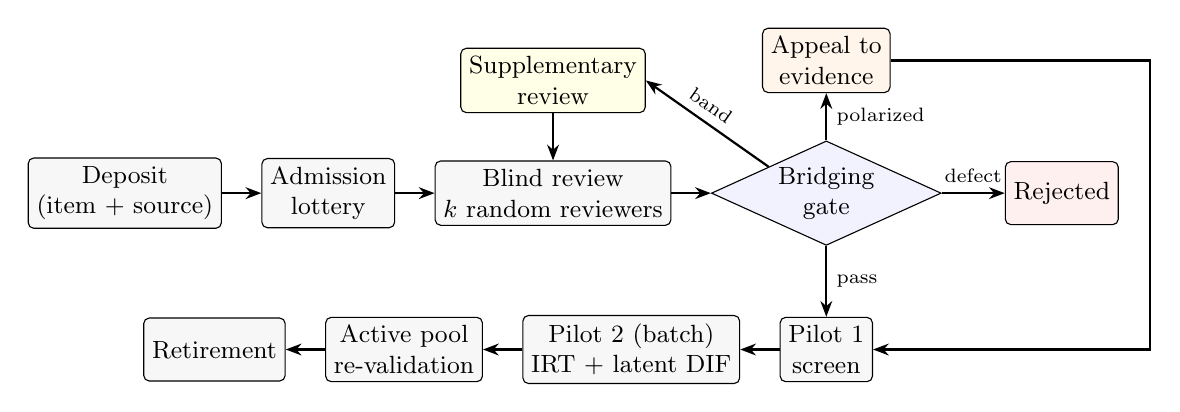
\begin{tikzpicture}[
  node distance=4mm and 5mm,
  box/.style={draw, rounded corners=2pt, align=center, font=\small, minimum height=8mm, inner sep=3pt, fill=gray!6},
  dec/.style={draw, diamond, aspect=2.2, align=center, font=\small, inner sep=1pt, fill=blue!5},
  arr/.style={-{Stealth[length=2mm]}, thick}]
\node[box] (dep) {Deposit\\(item + source)};
\node[box, right=of dep] (lot) {Admission\\lottery};
\node[box, right=of lot] (rev) {Blind review\\$k$ random reviewers};
\node[dec, right=of rev] (gate) {Bridging\\gate};
\node[box, below=9mm of gate] (p1) {Pilot 1\\screen};
\node[box, left=of p1] (p2) {Pilot 2 (batch)\\IRT + latent DIF};
\node[box, left=of p2] (pool) {Active pool\\re-validation};
\node[box, left=of pool] (ret) {Retirement};
\node[box, right=8mm of gate, fill=red!6] (rej) {Rejected};
\node[box, above=6mm of gate, fill=orange!8] (app) {Appeal to\\evidence};
\node[box, above=6mm of rev, fill=yellow!10] (band) {Supplementary\\review};
\draw[arr] (dep) -- (lot);
\draw[arr] (lot) -- (rev);
\draw[arr] (rev) -- (gate);
\draw[arr] (gate) -- node[right, font=\scriptsize]{pass} (p1);
\draw[arr] (gate) -- node[above, font=\scriptsize]{defect} (rej);
\draw[arr] (gate) -- node[right, font=\scriptsize]{polarized} (app);
\draw[arr] (gate.north west) -- node[above, font=\scriptsize, pos=0.55, sloped]{band} (band.east);
\draw[arr] (band.south) -- (rev.north);
\draw[arr] (app.east) -| ($(rej.east)+(4mm,0)$) |- (p1.east);
\draw[arr] (p1) -- (p2);
\draw[arr] (p2) -- (pool);
\draw[arr] (pool) -- (ret);
\end{tikzpicture}
\caption{Lifecycle of an item. Level~A (bridging) is only an upstream filter; the verdict comes
from the pilots (Level~B). A polarization rejection can be appealed directly to the pilots at the
cost of the author's reputation.}
\label{fig:pipeline}
\end{figure}

\section{Level A: bridging}\label{sec:levela}

\subsection{Model and estimator}

Let $\Omega\subseteq U\times J$ be the observed (reviewer, item) pairs of an epoch, with
$|U|=n$ reviewers and $|J|=m$ items, and let $r_{uj}\in[0,1]$ be the probability that
reviewer $u$ declares for item $j$. Each reviewer carries a weight $w_u\ge0$ computed from
the previous epoch: $0$ during probation, $1$ for the founders who bootstrap the network, and
$\min(w_{\max},E_u)$ afterwards, where $E_u$ is the evaluator score of \cref{sec:levelc}. The design then applies the anti-collusion discount of
\cref{sec:collusion}; the engine implements it, but the protocol does not yet apply it when it
computes these weights. The model is the
one-dimensional ($d=1$) factorization
\begin{equation}\label{eq:mf}
  \hat r_{uj} \;=\; \mu + \iota_u + \iota_j + f_u f_j ,
\end{equation}
with a global mean $\mu$, reviewer and item intercepts $\iota_u,\iota_j$ (written
$b_u,b_j$ in the repository), a reviewer position $f_u$ on a latent axis, and an item loading
$f_j$. The parameters $\xi=(\mu,\iota_U,\iota_J,f_U,f_J)$ minimize
\begin{equation}\label{eq:loss}
  L(\xi) = \sum_{(u,j)\in\Omega} w_u\,(r_{uj}-\hat r_{uj})^2
  + \lambda_b\Bigl(\sum_u \iota_u^2+\sum_j\iota_j^2\Bigr)
  + \lambda_f\Bigl(\sum_u f_u^2+\sum_j f_j^2\Bigr),
\end{equation}
with $\lambda_b=0.15$ and $\lambda_f=0.03$, and $\mu$ unpenalized. The objective is
non-convex. The reference implementation minimizes it with L-BFGS and a strong-Wolfe line
search~\cite{liu1989lbfgs,nocedal2006numerical} from eight seeded starts, keeps the lowest
objective, and fixes the sign of the axis by making the largest $|f_j|$ non-negative.

The \emph{bridge score} is pessimistic: $B_j=\min_s \iota_j^{(s)}$, taken over the full fit and
$10$ refits on subsamples that keep each observation with probability $0.85$~\cite{efron1993bootstrap}.
The gate compares $B_j$ with a threshold $\tau\approx0.08$ and a band half-width
$\varepsilon\approx0.008$, both provisional (\cref{sec:setting}).

The design rationale, taken from Community Notes~\cite{wojcik2022birdwatch}, is that heavy
penalties on the intercepts force the model to explain approval through the factor term first.
Approval that a reviewer's side alone explains goes into $f_uf_j$. Only approval that no side
explains, that is, approval \emph{across} the divide, survives in $\iota_j$. The rest of this
section examines what the objective actually guarantees.

\subsection{Invariances of the objective}

The data term of \eqref{eq:loss} depends on $\xi$ only through the predictions
$\hat r_{uj}$. Several transformations leave every prediction unchanged:
\begin{align*}
  &\text{(G1)}\;\; \mu\mapsto\mu+c,\;\; \iota_j\mapsto\iota_j-c\;\;\forall j;
  &&\text{(G2)}\;\; \mu\mapsto\mu+c,\;\; \iota_u\mapsto\iota_u-c\;\;\forall u;\\
  &\text{(G3)}\;\; f_u\mapsto f_u+c\;\;\forall u,\;\; \iota_j\mapsto\iota_j-c f_j\;\;\forall j;
  &&\text{(G4)}\;\; f_j\mapsto f_j+c\;\;\forall j,\;\; \iota_u\mapsto\iota_u-c f_u\;\;\forall u;\\
  &\text{(G5)}\;\; f_u\mapsto s f_u,\;\; f_j\mapsto f_j/s,\;\; s\neq0.
\end{align*}
(G3) translates the reviewers' axis and (G4) the items' axis; (G5) rescales the axis and, for
$s=-1$, flips its sign. Along these directions only the penalties vary, so the penalties alone
decide where the solution sits. This yields exact identities.

\begin{lemma}[Stationarity identities]\label{lem:gauge}\proved{}
For any weights $w_u\ge0$ and any stationary point of \eqref{eq:loss} (in particular any local
minimum),
\begin{align}
  &\textstyle\sum_j \iota_j = 0 \quad\text{and}\quad \sum_u \iota_u = 0, \label{eq:zerosum}\\
  &\textstyle\lambda_b\sum_j f_j\,\iota_j \;=\; \lambda_f\sum_u f_u, \label{eq:gauge-rev}\\
  &\textstyle\lambda_b\sum_u f_u\,\iota_u \;=\; \lambda_f\sum_j f_j, \label{eq:gauge-item}\\
  &\textstyle\sum_u f_u^2 \;=\; \sum_j f_j^2. \label{eq:scale}
\end{align}
\end{lemma}
\begin{proof}
Let $\xi^*$ be stationary and $\xi(c)$ a curve through it along one of the families above. The
data term is constant along the curve, so $0=\frac{d}{dc}L(\xi(c))|_{c=0}$ is the derivative of
the penalty alone. For (G1) this derivative is $-2\lambda_b\sum_j\iota_j$, and (G2) is
symmetric. For (G3) it is
$\frac{d}{dc}\bigl[\lambda_b\sum_j(\iota_j-cf_j)^2+\lambda_f\sum_u(f_u+c)^2\bigr]_{c=0}
=-2\lambda_b\sum_j f_j\iota_j+2\lambda_f\sum_u f_u$, and (G4) is symmetric. For (G5) it is
$\frac{d}{ds}\bigl[\lambda_f(s^2\sum_u f_u^2+s^{-2}\sum_j f_j^2)\bigr]_{s=1}
=2\lambda_f(\sum_u f_u^2-\sum_j f_j^2)$.
\end{proof}

On the repository's reference dataset (200 reviewers, 10 items, a 60/40 split between two
camps; \texttt{sim/bridging\_irt\_dif.py}), the best of eight fits has
$\|\nabla L\|_\infty=7\times10^{-7}$. Every identity holds to that precision:
$\sum_j\iota_j=1.9\times10^{-8}$, $\sum_u\iota_u=4.2\times10^{-6}$,
$\lambda_b\sum_jf_j\iota_j=\lambda_f\sum_uf_u=-3.899\times10^{-3}$,
$\lambda_b\sum_uf_u\iota_u=\lambda_f\sum_jf_j=6.426\times10^{-2}$ and
$\sum_uf_u^2=\sum_jf_j^2=8.568$.

Community Notes also penalizes $\mu$~\cite{wojcik2022birdwatch}. Identity~\eqref{eq:zerosum}
then becomes $\sum_j\iota_j=\mu$ (with a common penalty weight), a constraint that is negligible
when hundreds of thousands of notes are fitted jointly. Isegoria leaves $\mu$ unpenalized and
fits one epoch's batch of tens to hundreds of items, so the identity binds.

\subsection{The gate is relative to the batch}

\begin{proposition}[Batch relativity]\label{prop:zerosum}\proved{}
Let every term of the minimum defining $B_j$ be a stationary point of \eqref{eq:loss}. Then
$\sum_j B_j\le 0$. Hence the mean bridge score of every batch is non-positive, and if
$\tau-\varepsilon>0$, every batch contains an item below the band: no batch passes the gate in
full.
\end{proposition}
\begin{proof}
Fix one fit $s_0$ among those in the minimum. Then $B_j\le\iota_j^{(s_0)}$ for every $j$, and
$\sum_j\iota_j^{(s_0)}=0$ by \cref{lem:gauge}. If every $B_j\ge\tau-\varepsilon>0$, then
$\sum_jB_j>0$, a contradiction.
\end{proof}

The proposition says that the gate does not test ``is this item approved across the divide?''.
It tests ``is this item approved across the divide at least $\tau$ more than the average
item fitted with it?''. \Cref{tab:relativity} shows the effect on the repository's dataset. We
score six consensus items twice: inside the original ten-item batch, which also contains a
true but divisive item, two partisan items and one mildly partisan item, and alone.

\begin{table}[t]
\centering\small
\caption{Bridge scores $B_j$ of the six consensus items of the repository simulation, fitted
inside the original ten-item batch and fitted alone (same ratings, same estimator). Threshold
$\tau=0.08$. Source: \texttt{scripts/levelA\_relativity.py}.}
\label{tab:relativity}
\begin{tabular}{@{}lrrrrrr@{}}
\toprule
Item & 01 & 02 & 04 & 05 & 06 & 07\\
\midrule
In the ten-item batch & $+0.104$ & $+0.081$ & $+0.085$ & $+0.101$ & $+0.077$ & $+0.082$\\
Alone                 & $+0.014$ & $-0.017$ & $-0.001$ & $+0.011$ & $-0.022$ & $-0.014$\\
\midrule
Passes in batch / alone & yes/no & yes/no & yes/no & yes/no & no/no & yes/no\\
\bottomrule
\end{tabular}
\end{table}

\begin{finding}\label{find:relativity}\empirical{}
Five of the six consensus items pass when the batch contains divisive items and none passes
when they are scored together without them. Their approval did not change; the reference
point did.
\end{finding}

Three consequences follow. First, pass rates depend on the composition of the epoch. A
threshold ``calibrated on the pilot'', as the design prescribes, is calibrated to the pilot's
mix of items. Second, the design documents found that the reference value of Community Notes
(0.40) was unusable and that $\tau\approx0.08$ worked, and that scores ``cluster near the
threshold''. Both observations are consistent with batch-centred scores. Third, whoever
influences the composition of a batch influences who passes. For example, weak ``decoy''
items lower the batch average and raise the relative score of a target. The admission lottery
and the proposal rate limit bound this lever but do not remove it.

Three corrections are possible, and we have not evaluated any of them \openq. One is to penalize $\mu$
and fit many epochs jointly, which dilutes the constraint. Another is to anchor the scale with reference items of known standing and
express $\tau$ relative to them; the golden items that already enter every review queue
(\cref{sec:levelc}) could serve. The third is to declare the gate relative on purpose, as an
explicit quota. The second fits the rest of the design best.

\subsection{The origin of the axis decides how majoritarian the score is}

The translation (G3) moves the origin of the reviewer axis and trades item intercept against
loading. This matters because the position of the origin decides what ``approval not explained
by the axis'' means. We make this precise in a two-camp model.

Consider camps $A$ and $B$ with shares $\pi_A,\pi_B$ and imbalance
$\kappa=\pi_B-\pi_A\ge0$ (so $B$ is the majority). For item $j$ let $m_{Aj},m_{Bj}$ be the
camps' mean ratings, $\mbar_j=\tfrac12(m_{Aj}+m_{Bj})$ the \emph{camp-balanced} mean and
$\Delta_j=\tfrac12(m_{Bj}-m_{Aj})$ the item's lean. The \emph{camp-size-weighted} mean, which
is what a plain average of all ratings estimates, is $\pi_Am_{Aj}+\pi_Bm_{Bj}=\mbar_j+\kappa\Delta_j$.
We say a stationary point has the \emph{two-camp form} if:
\begin{enumerate}[label=(T\arabic*)]
  \item every reviewer of camp $s$ has $f_u=\varphi_s$ and $\iota_u=0$, with half-distance
    $h=\tfrac12(\varphi_B-\varphi_A)>0$ and midpoint $c=\tfrac12(\varphi_A+\varphi_B)$; and
  \item the fit reproduces the camp means: $\mu+\iota_j+\varphi_s f_j=m_{sj}$ for $s\in\{A,B\}$ and every $j$.
\end{enumerate}

\begin{proposition}[Majoritarian leak]\label{prop:leak}\proved{}
Let a stationary point of \eqref{eq:loss} have the two-camp form. Let $S=\sum_j\Delta_j^2$ and
$S_{\Delta m}=\sum_j\Delta_j(\mbar_j-\mu)$. Then:
\begin{enumerate}[label=(\roman*)]
  \item $f_j=\Delta_j/h$ and $\iota_j=\mbar_j-\mu-t\,\Delta_j$, where $t=c/h$ is the offset of
    the origin from the midpoint between the camps;
  \item $t=\dfrac{\lambda_b S_{\Delta m}-\lambda_f\,n h^2\kappa}{\lambda_b S+\lambda_f\,n h^2}$;
  \item if $S_{\Delta m}=0$, then
  \begin{equation}\label{eq:leak}
    \mu+\iota_j=(1-\ell)\,\mbar_j+\ell\,(\pi_Am_{Aj}+\pi_Bm_{Bj}),\qquad
    \ell=\frac{1}{1+\rho},\qquad \rho=\frac{\lambda_b S}{\lambda_f\,n\,h^2};
  \end{equation}
  \item and, in that case, $\rho=\dfrac{\lambda_b}{\lambda_f}\,\gamma\sqrt{S/n}$ for some
    $\gamma\in\bigl[\sqrt{1-\kappa^2},\,1\bigr]$.
\end{enumerate}
\end{proposition}
\begin{proof}
Part (i) follows from subtracting and averaging the two equations of (T2). For (ii),
substitute (i) and $\sum_uf_u=n_A\varphi_A+n_B\varphi_B=nh(t+\kappa)$ into
\eqref{eq:gauge-rev}, which gives $\lambda_b(S_{\Delta m}-tS)/h=\lambda_f\,nh\,(t+\kappa)$, and
solve for $t$. Part (iii) is (i) with $t=-\kappa/(1+\rho)$ from (ii). For (iv), \eqref{eq:scale}
gives $nh^2(1+t^2+2\kappa t)=S/h^2$. On $t\in[-\kappa,0]$ the factor $1+t^2+2\kappa t$ lies in
$[1-\kappa^2,1]$, so $h^2=\sqrt{S/(n(1+t^2+2\kappa t))}$, and substituting into the definition
of $\rho$ gives (iv).
\end{proof}

The \emph{leak} $\ell$ is the fraction of the majority's weight that passes into the bridge
score. At $\ell=0$ the score is camp-balanced: each camp counts once, whatever its size. This is
the property that motivates bridging. At $\ell=1$ the score is the size-weighted mean, which
is exactly what a plain average gives. The asymmetric penalty pushes $\ell$ toward $0$, but
$\lambda_b\gg\lambda_f$ is not the relevant condition. The relevant quantity is
$\rho\approx(\lambda_b/\lambda_f)\sqrt{S/n}$, which compares how stiffly the penalty holds the
item intercepts (summed over the batch's leans) with how stiffly it holds the reviewer positions
(summed over the reviewers). At a fixed ratio $\lambda_b/\lambda_f$, the leak grows with the
number of reviewers and falls only with the square root of the batch's total lean.

Assumptions (T1)--(T2) are idealizations. With regularization no fit is exact, and reviewers of a camp
do not share one position. \Cref{tab:leak} therefore tests \eqref{eq:leak} on the full model:
all parameters free, rating noise and reviewer severity as in the repository simulation,
within-camp spread of positions, and nine ratings per reviewer. The design uses mirror pairs:
ten consensus items and five pairs of partisan items with identical quality and opposite lean
($\Delta=\pm0.36$), camps of 60\% and 40\% ($\kappa=0.2$). The measured leak is
$(\iota_{P^+}-\iota_{P^-})/(2\kappa\Delta)$, which is $0$ for a camp-balanced score and $1$ for a
size-weighted one.

\begin{table}[t]
\centering\small
\caption{Majoritarian leak $\ell$ of the bridge score: measured on the full model (mean of three
datasets; standard deviation in parentheses) against the prediction $1/(1+\rho)$ of
\cref{prop:leak} with $\gamma=1$. Mirror-pair design, 60/40 camps. The default penalties are
$\lambda_b/\lambda_f=5$. Source: \texttt{scripts/levelA\_leak.py}.}
\label{tab:leak}
\pgfplotstabletypeset[
  col sep=comma,
  columns={ratio,N,leak_mean,leak_sd,predicted},
  columns/ratio/.style={column name={$\lambda_b/\lambda_f$},int detect},
  columns/N/.style={column name={reviewers $n$},int detect},
  columns/leak_mean/.style={column name={measured $\ell$},fixed,fixed zerofill,precision=2},
  columns/leak_sd/.style={column name={(sd)},fixed,fixed zerofill,precision=2,
    postproc cell content/.append style={/pgfplots/table/@cell content/.add={(}{)}}},
  columns/predicted/.style={column name={predicted $1/(1+\rho)$},fixed,fixed zerofill,precision=2},
  every head row/.style={before row=\toprule,after row=\midrule},
  every last row/.style={after row=\bottomrule},
  every row no 6/.style={after row=\midrule},
  every row no 13/.style={after row=\midrule},
]{data/levelA_leak.csv}
\end{table}

\begin{finding}\label{find:leak}\empirical{}
At the default penalties most of the camp-size effect survives in the bridge score: the leak is
0.53 with 50 reviewers and rises to 0.87 with 3{,}200. The closed form predicts every configuration within
0.1 and overestimates the leak in most of them; within-camp spread, absent from (T1), adds to
$\sum_uf_u^2$ and hence to $\rho$. Raising $\lambda_b/\lambda_f$ to 500 keeps the leak below 0.1
up to 3{,}200 reviewers.
\end{finding}

\begin{figure}[t]
\centering
\begin{tikzpicture}
\begin{semilogxaxis}[
  width=0.58\linewidth, height=5.2cm,
  xlabel={reviewers $n$}, ylabel={leak $\ell$},
  ymin=-0.05, ymax=1.0, xmin=40, xmax=4000,
  legend style={font=\scriptsize, at={(1.03,1)}, anchor=north west, draw=none, fill=none},
  grid=major, grid style={gray!20}, tick label style={font=\scriptsize}, label style={font=\small}]
\addplot[only marks, mark=*, mark size=1.6pt, color=blue!70!black, skip coords between index={7}{21}]
  table[col sep=comma, x=N, y=leak_mean] {data/levelA_leak.csv};
\addlegendentry{$\lambda_b/\lambda_f=5$}
\addplot[only marks, mark=square*, mark size=1.5pt, color=orange!80!black, skip coords between index={0}{7}, skip coords between index={14}{21}]
  table[col sep=comma, x=N, y=leak_mean] {data/levelA_leak.csv};
\addlegendentry{$\lambda_b/\lambda_f=50$}
\addplot[only marks, mark=triangle*, mark size=1.8pt, color=green!45!black, skip coords between index={0}{14}]
  table[col sep=comma, x=N, y=leak_mean] {data/levelA_leak.csv};
\addlegendentry{$\lambda_b/\lambda_f=500$}
\addplot[thick, color=blue!70!black, forget plot, skip coords between index={7}{21}]
  table[col sep=comma, x=N, y=predicted] {data/levelA_leak.csv};
\addplot[thick, color=orange!80!black, forget plot, skip coords between index={0}{7}, skip coords between index={14}{21}]
  table[col sep=comma, x=N, y=predicted] {data/levelA_leak.csv};
\addplot[thick, color=green!45!black, skip coords between index={0}{14}]
  table[col sep=comma, x=N, y=predicted] {data/levelA_leak.csv};
\addlegendentry{prediction $1/(1+\rho)$ (lines)}
\end{semilogxaxis}
\end{tikzpicture}
\caption{Majoritarian leak against the number of reviewers (points: full model; lines:
$1/(1+\rho)$ from \cref{prop:leak}). Data as in \cref{tab:leak}.}
\label{fig:leak}
\end{figure}

\Cref{prop:leak} also explains an asymmetry in the repository simulation. There $n=200$,
$S\approx0.39$ and $\kappa=0.2$, so $\rho\approx0.22$ and $\ell\approx0.82$. The majority's
partisan item and the minority's mirror-image item have the same quality and opposite lean. In
the full fit they score $-0.155$ and $-0.260$. The proposition predicts a gap of
$\ell\kappa(\Delta_{08}-\Delta_{09})\approx0.82\times0.2\times0.72\approx0.12$; the measured
gap is $0.105$. Both items fail here. For items closer to $\tau$, however, which of two mirror
images passes depends on which camp is larger, which is what bridging is meant to prevent.

The normative content of bridging, ``each side counts once'', therefore sits in a gauge. The
objective reaches it only in the limit $\rho\to\infty$, and with more than two groups or a
continuum of positions the ``midpoint'' is itself a choice. We see three remedies
\openq:
\begin{enumerate}[label=(\alph*)]
  \item scale the penalty ratio with $\sqrt{n/S}$; for example, $\rho\ge9$ keeps $\ell\le0.1$;
  \item fix the gauge explicitly, for instance by imposing $\sum_jf_j\iota_j=0$, the
    $\rho\to\infty$ limit of \eqref{eq:gauge-rev}. The origin then depends on $S_{\Delta m}$, the
    correlation between lean and approval within the batch, which is a new lever for anyone
    who controls the batch's composition;
  \item replace the intercept by a gauge-invariant statistic of the predictions, such as the
    smaller of the mean predicted ratings $\hat r_{uj}$ among reviewers in the lowest and in the
    highest decile of $f_u$. Predictions are invariant under (G1)--(G5), so any function of
    them is too, and a minimum across the spectrum does not depend on camp sizes.
\end{enumerate}

\subsection{What ratings cannot distinguish}

\begin{proposition}[Observational equivalence]\label{prop:equivalence}\proved{}
Let $D$ be any decision rule, deterministic or randomized, that depends on the data only
through the assignment $\Omega$ and the ratings $(r_{uj})$. If two items induce the same
distribution of ratings from every reviewer, then $D$ has the same distribution of outcomes on
both.
\end{proposition}
\begin{proof}
The distribution of $D$'s output is a function of the joint distribution of its inputs, which is
the same for both items.
\end{proof}

The proposition is elementary, but it settles the most serious limitation of Level~A. A true
fact that one camp rejects and a false claim that the other camp accepts can polarize the same
camps in the same way. When they do, no function of the ratings separates them, and every
threshold trades lost true items for admitted partisan ones. The repository simulation shows
this: at every $\tau$ in $[0.02,0.12]$ the true but divisive item fails, while no partisan item
passes. The remedy has to bring in information the ratings do not contain. That is the role of
the appeal to evidence, which sends a polarization rejection to the pilots at the author's risk.
\Cref{sec:dif-not-bias} discusses how far that remedy reaches.

\subsection{Capture cost in the reference simulation}

In the repository simulation, 40 members of the majority camp rate the majority's partisan
item at $1$, and members of the opposing camp are added one group at a time. The bridge score
moves from $-0.14$ (no opposing raters) through $-0.10$, $-0.06$, $-0.02$, $+0.02$ and $+0.07$ to
$+0.13$ (10, 20, 30, 40, 55 and 70 opposing raters). The crossing of $\tau=0.08$ therefore lies
between 55 and 70 of the 80 opposing reviewers (69--88\%); linear interpolation gives about 57
(71\%). The design documents quote ``70 of 80 (87\%)'', which is the upper end of this bracket
\empirical. This is one dataset and one seed. A capture-cost curve with confidence bands is
part of the evaluation plan (\cref{sec:plan}). \Cref{prop:leak} adds that votes from the
majority's own camp are not neutralized: they act through the leak.

\subsection{Further identifiability conditions}

The sign of the axis is fixed as described above. If the bipartite graph of $\Omega$ is
disconnected, each component has its own gauge and the scores of different components are not
comparable. Random assignment with $k\ge7$ reviewers per item makes this unlikely, but the
engine does not check it. The specification states that reviewers with fewer than $n_{\min}=30$
ratings should not define the axis. This rule and the two-dimensional model are not
implemented; the second is deferred by design decision D31~\cite{isegoria-repo}.

\section{Level B: evidence}\label{sec:levelb}

Level~B decides. Items that pass the gate, or that are appealed, are trialled on respondents
who answer them mixed with validated items. The verdict comes from the responses alone.

\subsection{Ability and item screening}

Respondent $i$'s ability is estimated as $\theta_i=(T_i-\bar T)/\mathrm{sd}(T)$, the
standardized total score over a set of anchor items already certified free of DIF (30 in the
repository simulations). For each trial item, a two-parameter logistic model
(2PL)~\cite{birnbaum1968,lord1980}
\begin{equation}\label{eq:2pl}
  P(X_{ij}=1\mid\theta_i)=\sig\bigl(a_j(\theta_i-b_j)\bigr),
\end{equation}
is fitted by logistic regression on the fixed $\theta$, giving a discrimination $a_j$ and a
difficulty $b_j$. A fit that does not converge, for example under complete separation, is
treated as undetermined. Stage~1 of the pilot keeps an item if its point-biserial correlation
with $\theta$ is at least $0.20$, its fit converged, and $a_j\ge0.6$. A negative point-biserial
reveals an inverted answer key, and the simulations catch one. Two gaps are acknowledged in the
repository and remain open \openq. First, $\theta$ is a proxy on the standardized-total metric,
while the thresholds come from a literature that uses an IRT metric~\cite{hambleton1991}.
Second, no guessing parameter is fitted, although multiple-choice items with four options are
exactly where guessing matters (design decision D25).

\subsection{DIF with observed groups: calibration only}

With an observed group $g_i\in\{-1,+1\}$, DIF is tested by the logistic
model~\cite{swaminathan1990}
$\logit P(X_{ij}=1)=\beta_0+\beta_1\theta_i+\beta_2g_i+\beta_3\theta_ig_i$, rejecting at
$|\beta_2|>0.40$, and by the Mantel--Haenszel common odds ratio with the ETS
classes~\cite{mantel1959,holland1988mh,zieky1993}. Both need a per-respondent group label.
\Cref{req:anon} forbids that label in production, so these tests are compiled only into closed
calibration pilots with declared attributes (design decision D20). Production uses the latent
variant below.

\subsection{DIF on latent classes}

The anonymity-compatible detector is a mixture IRT model~\cite{rost1990,cohen2005mixture}. Each
respondent belongs to an unobserved class $Z_i\in\{1,\dots,G\}$ with proportions $\pi_g$, and
responses are independent given $(\theta_i,Z_i)$:
\begin{equation}\label{eq:mixture}
  P(X_{ij}=1\mid\theta_i,Z_i=g)=\sig\bigl(a_{jg}(\theta_i-b_{jg})\bigr),\qquad
  \ell(\cdot)=\sum_i\log\sum_g\pi_g\prod_j P(x_{ij}\mid\theta_i,g).
\end{equation}
The implementation tries $G\in\{1,\dots,4\}$, each with a shared discrimination
($a_{jg}=a_j$, uniform DIF) and with a per-class one. Every candidate is fitted from seeded
starts with an analytic gradient, and the candidate with the lowest
BIC~\cite{schwarz1978} is kept. The search stops once an extra class no longer lowers the BIC.
The item statistic is $\mathrm{DIF}_j=\max_{g,h}|b_{jg}-b_{jh}|$ over classes holding at least 5\%
of the respondents. An item is flagged if the selected fit converged, has at least two classes,
and $\mathrm{DIF}_j>1.0$. The literature value for this gap is $0.5$. The repository reports
that $0.5$ flags every item of a batch with one biased item, keeps $1.0$ as provisional, and
defers the choice to a planned false-positive study. Batches must hold at least two items and
3{,}000 respondents. Mixture likelihood ratios are not $\chi^2$-distributed under the
null~\cite{self1987,mclachlan2000}, so the BIC comparison is a heuristic, not a calibrated test.

\subsection{Identification: why a single biased item is invisible}

The repository simulation found that one distorted item in a batch of eight is invisible and
two are detected. The following two propositions explain this.

\begin{proposition}[One class-dependent item]\label{prop:single}\proved{}
Let $\theta$ be observed without error and $Z$ independent of $\theta$, and suppose only item
$j$'s response function depends on $Z$. Then the likelihood factorizes as
$\prod_{k\neq j}P_k(x_k\mid\theta)\cdot\bigl[\sum_g\pi_gP_{jg}(x_j\mid\theta)\bigr]$, so the
class parameters are identified only through the marginal response curve
$m_j(\theta)=\sum_g\pi_g\,\sig(a_{jg}(\theta-b_{jg}))$. For a symmetric two-class shift
($\pi=\tfrac12$, $b_{j\pm}=b_j\pm\delta$, common $a$), with $x=a(\theta-b_j)$,
\begin{equation}\label{eq:single-expansion}
  m_j(\theta)=\sig(x)+\tfrac12(a\delta)^2\sig''(x)+O(\delta^4)
  =\sig\bigl((1-\tfrac14(a\delta)^2)\,x\bigr)
   +\tfrac12(a\delta)^2\,\sig'(x)\bigl(\tfrac{x}{2}-\tanh\tfrac{x}{2}\bigr)+O(\delta^4).
\end{equation}
\end{proposition}
\begin{proof}
With only item $j$ depending on $Z$, summing over $Z$ acts on item $j$'s factor alone. The
expansion averages $\sig(x\pm a\delta)$, so odd orders cancel. It then uses
$\sig''(x)=-\sig'(x)\tanh(x/2)$ and $\sig((1+\eta)x)=\sig(x)+\eta x\sig'(x)+O(\eta^2)$ with
$\eta=-\tfrac14(a\delta)^2$.
\end{proof}

In words, a single class-dependent item looks, to second order, like a 2PL item with a lower
discrimination. The residual $\tfrac{x}{2}-\tanh\tfrac{x}{2}=x^3/24+O(x^5)$ vanishes to third
order where the item is most informative. The same flattening is produced by error in
$\theta$, so the two are confounded in practice.

\begin{proposition}[Pairs of class-dependent items]\label{prop:pair}\proved{}
Under conditional independence given $(\theta,Z)$,
\begin{equation}\label{eq:pair-cov}
  \Cov(X_j,X_k\mid\theta)=\sum_g\pi_g\,\bigl(P_{jg}(\theta)-m_j(\theta)\bigr)\bigl(P_{kg}(\theta)-m_k(\theta)\bigr),
\end{equation}
which for two classes equals $\pi(1-\pi)\,\Delta_j(\theta)\Delta_k(\theta)$ with
$\Delta_j=P_{j2}-P_{j1}$. Any one-class model implies $\Cov(X_j,X_k\mid\theta)=0$. Hence two items
whose class-dependence overlaps in $\theta$ leave a signature that no one-class model absorbs.
\end{proposition}
\begin{proof}
$\E[X_jX_k\mid\theta]=\sum_g\pi_gP_{jg}P_{kg}$ and $\E[X_j\mid\theta]=m_j$. Expanding the
covariance gives \eqref{eq:pair-cov}. For two classes, substitute $m_j=(1-\pi)P_{j1}+\pi P_{j2}$.
\end{proof}

Both signals are of fourth order in $\delta$ for small $\delta$, but their constants differ
greatly. \Cref{tab:information} gives the expected likelihood-ratio contribution
($2N\times$ the per-respondent information) at $N=3000$. For one item, this is the minimal
expected Kullback--Leibler divergence between the mixture curve and any 2PL. For a pair, it is
the conditional mutual information $I(X_j;X_k\mid\theta)$.

\begin{table}[t]
\centering\small
\caption{Expected likelihood-ratio contribution at $N=3000$ of one biased item (the part no 2PL
absorbs) and of one biased pair (conditional mutual information), for $a=1.25$, $b=0$,
$\pi=\tfrac12$ and exact $\theta$. For comparison, the BIC penalty per extra parameter is
$\ln 3000\approx8$. Source: \texttt{scripts/levelB\_information.py}.}
\label{tab:information}
\pgfplotstabletypeset[
  col sep=comma,
  columns={delta,lr_single,lr_pair,ratio},
  columns/delta/.style={column name={shift $\delta$},fixed,fixed zerofill,precision=2},
  columns/lr_single/.style={column name={one biased item},fixed,fixed zerofill,precision=3},
  columns/lr_pair/.style={column name={one biased pair},fixed,fixed zerofill,precision=2},
  columns/ratio/.style={column name={ratio},fixed,precision=0},
  every head row/.style={before row=\toprule,after row=\midrule},
  every last row/.style={after row=\bottomrule},
]{data/levelB_information.csv}
\end{table}

\begin{finding}\label{find:information}\empirical{}
A biased pair carries 245--306 times the information of a single biased item. At $\delta=0.9$
and $N=3000$, a single item contributes $0.5$ to the expected likelihood ratio, far below any
penalty, while a pair contributes $130$. The repository simulation, which uses a proxy $\theta$,
measures about $100$ per biased pair. For small shifts, pairwise information scales as
$\approx0.048\,\delta^4$ per respondent (the constant falls to $0.033$ at $\delta=0.9$, where the
classes start to separate), so halving the shift requires about sixteen times the respondents for
the same power. The production detector agrees. With exact $\theta$ it selects no mixture in 8
null batches and detects nothing in 8 batches with one biased item ($N\in\{3000,6000\}$), and it
flags exactly the biased items in all 8 batches with two, with no false flag.
\end{finding}

\Cref{prop:single,prop:pair} turn \cref{req:batch} from an empirical rule into a structural one.
The latent classes are identified by \emph{covariation between items} given ability, so they need
at least two items that share a distortion. A campaign to tilt the bank leaves this signature. An
isolated distortion does not, and neither does a single biased item repeated across batches that
never contain another item biased the same way.

\subsection{A confound: error in the ability proxy}\label{sec:proxy}

The detector conditions on $\hat\theta$, a standardized anchor total, not on $\theta$.

\begin{proposition}[Proxy-induced dependence]\label{prop:proxy}\proved{}
Let $\hat\theta$ be computed from anchor responses that are independent of the trial items
given $\theta$, and let every trial item's response function be non-decreasing in $\theta$.
Then, with no DIF at all,
\begin{equation}
  \Cov(X_j,X_k\mid\hat\theta)=\Cov\bigl(P_j(\theta),P_k(\theta)\bigm|\hat\theta\bigr)\;\ge\;0,
\end{equation}
with strict inequality whenever $\Var(\theta\mid\hat\theta)>0$ and both functions are strictly
increasing.
\end{proposition}
\begin{proof}
Conditional independence gives $\E[X_jX_k\mid\hat\theta]=\E[P_j(\theta)P_k(\theta)\mid\hat\theta]$
and $\E[X_j\mid\hat\theta]=\E[P_j(\theta)\mid\hat\theta]$. Two non-decreasing functions of the
same random variable are non-negatively correlated (Chebyshev's association inequality), and
strictly so if both are strictly increasing and the variable is not degenerate.
\end{proof}

Local dependence therefore exists whenever the proxy is imperfect, with or without DIF. A
mixture whose classes shift all items in the same direction absorbs part of it, as a ``higher
than measured'' and a ``lower than measured'' class. The likelihood ratio then grows linearly
in $N$, while the BIC penalty grows like $\ln N$, so for large enough samples the BIC selects a
mixture on data that contain none. The estimated gap of \emph{every} item then equals the size of
the common shift. This is the observed-score version of a problem known in DIF research:
matching on an unreliable total inflates DIF, which is why SIBTEST corrects the matching
variable by regression~\cite{shealy1993sibtest}.

\begin{table}[t]
\centering\small
\caption{Likelihood ratio of the two-class uniform-DIF mixture against one class, with $\theta$
from 30 anchors (proxy) or exact, for batches of 8 items of which 0, 1 or 2 are biased
($\delta=0.9$). Mean of three datasets. Last row: BIC penalty $8\ln N$ used by the repository
simulation. Source: \texttt{scripts/levelB\_proxy.py}.}
\label{tab:proxy}
\begin{tabular}{@{}llrrrr@{}}
\toprule
$\theta$ & biased items & $N=1500$ & $3000$ & $6000$ & $12000$\\
\midrule
proxy & 0 & 53.7 & 91.2 & 169.0 & 281.9\\
proxy & 1 & 48.2 & 84.5 & 152.7 & 239.3\\
proxy & 2 & 67.1 & 219.7 & 433.4 & 568.8\\
\midrule
exact & 0 & 15.5 & 17.8 & 15.9 & 20.0\\
exact & 1 & 13.6 & 12.1 & 18.9 & 18.2\\
exact & 2 & 47.8 & 170.2 & 324.1 & 419.1\\
\midrule
\multicolumn{2}{@{}l}{penalty $8\ln N$} & 58.5 & 64.1 & 69.6 & 75.1\\
\bottomrule
\end{tabular}
\end{table}

\Cref{tab:proxy} shows the effect in a re-implementation of the repository simulation's model.
With exact $\theta$ the likelihood ratio stays flat when there is nothing to find, and also when
there is one biased item, as \cref{prop:single} predicts. With the proxy it grows linearly in
$N$ even with zero biased items, and it exceeds the penalty from $N=3000$ on. The mean
estimated gap of clean items is then $0.71$--$0.86$.

To measure the consequence for the production detector, we ran the Rust engine and the
protocol's verdict rule on null batches (no biased item, $N=6000$) whose $\theta$ comes from 10,
20, 30 or 60 anchors (\cref{tab:anchors}).

\begin{table}[t]
\centering\small
\caption{Production detector (Rust engine and verdict rule) on null batches: eight clean items,
$N=6000$, four datasets per row, $\theta$ from the stated number of anchors. A flag here is a
false positive. Source: \texttt{scripts/levelB\_detector.py}.}
\label{tab:anchors}
\begin{tabular}{@{}rcccc@{}}
\toprule
anchors & mixture selected & largest clean gap & batches with a false flag & items flagged per batch\\
\midrule
10 & 4/4 & 1.27--1.41 & 4/4 & 8 of 8\\
20 & 4/4 & 1.04--1.16 & 4/4 & 1--3\\
30 & 4/4 & 0.94--0.99 & 0/4 & 0\\
60 & 0/4 & --- & 0/4 & 0\\
\bottomrule
\end{tabular}
\end{table}

\begin{finding}\label{find:proxy}\empirical{}
On null batches the production detector selects a spurious mixture whenever the proxy is
imperfect enough. With 10 or 20 anchors it flags clean items in every batch. With 30 anchors,
the configuration of the repository simulations, it flags none, but the largest clean gap
reaches $0.94$--$0.99$ against a threshold of $1.0$. The provisional threshold is therefore
calibrated, implicitly, to one anchor configuration. With the same 30 anchors and one biased
item at $N=6000$, the detector flags the biased item in 2 of 4 batches (gaps $1.15$ and $1.03$).
It does so because the item rides on the artefactual class, not because its own shift is
identified; with exact $\theta$ it is never detected.
\end{finding}

Three remedies are available \openq.
\begin{enumerate}[label=(\alph*)]
  \item Put the anchors inside the likelihood with class-invariant parameters and integrate
    $\theta$ out, which gives a full mixture IRT model. The anchors then identify class-specific
    ability distributions, and a class-wide shift is no longer mistaken for DIF. This is the
    principled fix. Its cost is computational.
  \item Allow a class-specific ability shift and measure each item's departure from the batch's
    common class shift. In the two-class parametrization $b_{j\pm}=b_j\pm\delta_j$ of the
    repository simulation this is $2|\delta_j-\operatorname{median}_k\delta_k|$. In our re-implementation
    this ``differential gap'' separates biased items (at least $1.65$) from clean ones (at most
    $0.32$) at both sample sizes, with 30 anchors
    (\texttt{scripts/levelB\_differential.py}). A campaign that biases most of a batch in
    one direction would, however, be absorbed into the common shift, so this can only
    complement (a).
  \item At a minimum, make the threshold a documented function of anchor reliability and
    calibrate it by simulation, as the evaluation plan requires.
\end{enumerate}

\subsection{Sample sizes and the minimum network}

The pilot sizes of about $300$ (screen) and $1500$--$3000$ (DIF) are calibration targets taken
from the psychometric literature, not derived results. The repository labels them a
hypothesis \openq. \Cref{find:information} gives a first handle: for small shifts a biased pair
contributes an expected likelihood ratio of about $2N\times0.048\,\delta^4$ for $a\approx1.25$. Detection needs
this to exceed the penalty of the extra class, which is roughly $(K+1)\ln N$ for a batch of $K$
items. The respondent requirement sets a floor on the network's size. A batch needs a few
thousand \emph{distinct} respondents in its validation window, and anonymity is weak in a small
crowd. The repository estimates that the network cannot run as specified below about $2{,}000$
active participants.

\subsection{DIF is not bias}\label{sec:dif-not-bias}

DIF shows that, at equal measured ability, an item's difficulty depends on something else: the
item measures a secondary dimension on which the classes differ~\cite{shealy1993sibtest}.
Whether that secondary dimension is a nuisance is a judgment, not a statistical fact. For civic
knowledge the judgment matters. Suppose one camp is systematically misinformed about a
true fact. Then an item stating that fact shows DIF by construction, and Level~B rejects it for
the same reason Level~A did. The appeal to evidence therefore recovers a true but divisive item
only when the division lies in \emph{opinions about the item}, and not when it lies in
\emph{knowledge of the fact}. The design currently treats every politically aligned secondary
dimension as a nuisance. That is a normative choice, and we argue it should be made explicitly
\designchoice. The same mechanism detects distortions on axes nobody chose to look for. In the
repository simulation, an item neutral on the political axis shows DIF of $0.66$ on education.
Latent classes can surface such an axis, but only when a batch contains at least two items
distorted along it.

\section{Level C: reputation}\label{sec:levelc}

Reputation enters in two separate scores on unlinkable pseudonyms (\cref{req:separate}). The
author score limits how much an author may propose. The evaluator score weights reviews.

\subsection{Author score}

Let $q_j\in[0,1]$ be the final quality of author $a$'s item $j$, a function of its Level~B
statistics whose exact definition is still open. The author score is the shrunken, time-discounted
average
\begin{equation}\label{eq:author}
  C_a=\frac{\alpha_0+\sum_j w_jq_j}{\alpha_0+\beta_0+\sum_j w_j},\qquad w_j=e^{-\Delta t_j/T},
\end{equation}
with prior $(\alpha_0,\beta_0)=(2,3)$ and $T=18$ months. Two accepted items out of two give
$4/7\approx0.57$; 180 out of 200 give $182/205\approx0.89$. $C_a$ sets the proposal rate
$q_{\min}+(q_{\max}-q_{\min})C_a$. It never weights a vote \designchoice. A failed appeal to
evidence is to be recorded as a negative pseudo-observation inside $C_a$, escrowed when the appeal
is filed (design decision D27). The reference implementation still applies a simpler
stake-and-refund rule.

\subsection{Evaluator score: forecasts scored on golden items}

Every reviewer declares a probability $p_{uj}$ that item $j$ will pass empirical validation. The
same number is the rating $r_{uj}$ of Level~A. About 5\% of every review queue consists of
\emph{golden} items. These are indistinguishable from the rest, and their outcome
$o_j\in\{0,1\}$ is known from validated history (design decision D21). The forecasts on golden
items are scored. The design goal (design decision D6) is that honest forecasting is optimal, that
copying the crowd earns nothing, and that being right where the crowd is wrong is what pays. Its
opposite would be a Schelling-point mechanism that rewards agreement with the majority. The
current rule is the Brier skill score against the crowd~\cite{brier1950,murphy1988skill}:
\begin{equation}\label{eq:bss}
  \mathrm{BSS}_u=1-\frac{\sum_j(p_{uj}-o_j)^2}{\sum_j(\bar p_j-o_j)^2},\qquad
  \bar p_j=\frac{\sum_v w_vp_{vj}}{\sum_v w_v},
\end{equation}
where the crowd forecast $\bar p_j$ averages the whole panel, the reviewer included (design
decision D23). The evaluator score is $E_u=\sig(\gamma\,\mathrm{BSS}_u)$. It is updated by an
asymmetric moving average that rises slowly and falls fast, and it gives the weight
$w_u=\min(w_{\max},E_u)$ with $w_{\max}=3\operatorname{median}(w)$.

Scoring only golden items is more than a convenience. On a live item the outcome is observed only
if the item reaches Level~B, and whether it does depends on the forecasts themselves, because they
are also the bridging ratings. When a forecast influences whether its outcome is observed, known
results on decision scoring show that strict properness requires randomizing the
decision~\cite{othman2010decision,chen2014eliciting}.
Golden items avoid the problem because their outcome is fixed in advance.

\subsection{The ratio-form skill score is not proper}

\begin{proposition}[Non-properness of the skill score]\label{prop:bss}\proved{}
Score a single item with baseline $b\in(0,1)$ that does not depend on the report, and let the
reviewer believe $P(o=1)=q\in(0,1)$. The expected skill score
\[
  \E[\mathrm{BSS}]=1-\frac{q(1-p)^2}{(1-b)^2}-\frac{(1-q)\,p^2}{b^2}
\]
is strictly concave in $p$, and its maximizer satisfies
\begin{equation}\label{eq:bss-opt}
  \logit p^{*}=\logit q+2\logit b .
\end{equation}
Truthful reporting is optimal if and only if $b=\tfrac12$.
\end{proposition}
\begin{proof}
The expectation over $o$ is immediate. The first-order condition
$q(1-p)/(1-b)^2=(1-q)p/b^2$ gives $p/(1-p)=\frac{q}{1-q}\cdot\frac{b^2}{(1-b)^2}$, which is
\eqref{eq:bss-opt}. The second derivative is $-2q/(1-b)^2-2(1-q)/b^2<0$.
\end{proof}

That skill scores built on a proper score are themselves improper, and that the resulting hedging
shrinks as the number of scored forecasts grows, is known in forecast
verification~\cite{murphy1973hedging}. What matters here is the direction of the hedge. A ratio of
two random sums is not an expectation of a score. The denominator gives more weight to outcomes
where the crowd was right, and \eqref{eq:bss-opt} shows the result: the report is pushed
toward the outcome the crowd favours, by twice the crowd's log-odds. With the crowd at $0.65$,
a reviewer who believes $0.78$ should report $0.92$, and a reviewer who believes $0.30$ should
report $0.60$, crossing to the crowd's side (\cref{fig:bss}). The distortion is largest for the
dissenter, who is exactly the reviewer the design wants to reward.

\begin{figure}[t]
\centering
\begin{tikzpicture}
\begin{axis}[
  width=0.62\linewidth, height=5.6cm,
  xlabel={belief $q$}, ylabel={optimal report $p^*$},
  xmin=0, xmax=1, ymin=0, ymax=1,
  legend style={font=\scriptsize, at={(0.98,0.03)}, anchor=south east, draw=none, fill=white, fill opacity=0.8, text opacity=1},
  grid=major, grid style={gray!20}, tick label style={font=\scriptsize}, label style={font=\small}]
\addplot[gray, dashed, domain=0:1] {x};
\addlegendentry{truthful}
\addplot[thick, blue!70!black] table[col sep=comma, x=q, y=pstar_fixed] {data/levelC_bss_curve.csv};
\addlegendentry{BSS, baseline $0.65$ (closed form)}
\addplot[thick, orange!85!black, densely dotted] table[col sep=comma, x=q, y=pstar_selfincl] {data/levelC_bss_curve.csv};
\addlegendentry{BSS, baseline includes the reviewer}
\addplot[only marks, mark=*, mark size=1.8pt, red!70!black] coordinates {(0.30,0.5965)};
\end{axis}
\end{tikzpicture}
\caption{Report that maximizes the expected Brier skill score on one golden item, against the
reviewer's belief, when the other panelists' mean forecast is $0.65$. Solid line: baseline
excluding the reviewer (\cref{prop:bss}). Dotted line: baseline including the reviewer with
weight $1/9$, as in the implementation (numerical). The marked point is a dissenter who
believes $0.30$ and is best off reporting $0.60$. Source: \texttt{scripts/levelC\_bss.py}.}
\label{fig:bss}
\end{figure}

With several items the ratio couples them, and there is no closed form. \Cref{tab:bss} gives the
exact optimum, enumerating all $2^m$ outcomes, for random beliefs and baselines.

\begin{table}[t]
\centering\small
\caption{Distortion of the optimal report under the ratio-form skill score, $|p^*_j-q_j|$,
for $m$ jointly scored items with beliefs uniform on $[0.1,0.9]$ and baselines uniform on
$[0.2,0.8]$ (200 random instances; 60 for $m=8$). Source: \texttt{scripts/levelC\_bss.py}.}
\label{tab:bss}
\begin{tabular}{@{}rcccc@{}}
\toprule
& \multicolumn{2}{c}{baseline: others only} & \multicolumn{2}{c}{baseline includes reviewer}\\
\cmidrule(lr){2-3}\cmidrule(l){4-5}
$m$ & mean & max & mean & max\\
\midrule
1 & 0.229 & 0.577 & 0.227 & 0.569\\
2 & 0.127 & 0.434 & 0.118 & 0.416\\
4 & 0.061 & 0.173 & 0.061 & 0.227\\
8 & 0.030 & 0.081 & 0.035 & 0.095\\
\bottomrule
\end{tabular}
\end{table}

\begin{finding}\label{find:bss}\empirical{}
The mean distortion falls roughly as $0.23/m$ in the number of jointly scored golden items,
consistent with Murphy's observation. Including the reviewer in the baseline, as the
implementation does, changes it little. At a golden-item rate of 5\%, a reviewer who judges about
ten items per epoch meets a golden item about every other epoch. A score computed over a few
golden items is therefore in the regime of the largest distortion.
\end{finding}

\subsection{A proper alternative}

\begin{proposition}[Leave-one-out difference score]\label{prop:loo}\proved{}
Let $\bar p_{-u,j}$ be the weighted mean forecast of the \emph{other} panelists on item $j$, and
\begin{equation}\label{eq:loo}
  S_u=\frac1m\sum_{j}\Bigl[(\bar p_{-u,j}-o_j)^2-(p_{uj}-o_j)^2\Bigr].
\end{equation}
Under \cref{ass:blind}, so that $\bar p_{-u,j}$ does not depend on $p_{uj}$:
\begin{enumerate}[label=(\roman*)]
  \item $S_u$ is strictly proper: $\E[S_u]=c_u-\frac1m\sum_j(p_{uj}-q_j)^2$ with $c_u$ not
    depending on the reports, so truthful reporting is the unique optimum;
  \item a reviewer who copies the crowd ($p_{uj}=\bar p_{-u,j}$) scores exactly $0$ for every
    outcome, not only in expectation;
  \item $S_u>0$ if and only if the reviewer's Brier score on the scored items beats the crowd's;
  \item $S_u$ is additive over items, so it aggregates across epochs without reweighting.
\end{enumerate}
\end{proposition}
\begin{proof}
For (i), use $\E[(p-o)^2]=(p-q)^2+q(1-q)$ for $o\sim\mathrm{Bernoulli}(q)$~\cite{gneiting2007scoring}.
Parts (ii)--(iv) are immediate from \eqref{eq:loo}.
\end{proof}

The difference score keeps what D6 wants from the skill score, namely zero for copying the crowd
and a positive score only for beating it, and drops the ratio that breaks properness. One new
exposure deserves mention. Because the baseline is formed by the other panelists, a coalition can
raise a member's score by degrading its own forecasts. This costs the saboteurs their own scores,
is bounded by their share of the panel weight, and is blunted by the fact that golden items are
indistinguishable from live ones, whose ratings also enter bridging.

\subsection{From scores to weights}

\begin{proposition}[A cap that never binds]\label{prop:cap}\proved{}
If all weights lie in $(0,1)$ and $\operatorname{median}(w)\ge\tfrac13$, then
$w_{\max}=3\operatorname{median}(w)\ge1>w_u$ for every $u$, so $\min(w_{\max},E_u)=E_u$ always.
\end{proposition}

With $E_u=\sig(\gamma\,\mathrm{BSS}_u)$ and a crowd baseline that puts the typical reviewer's
score near zero, the median of $E$ is close to $\tfrac12$, so the cap is vacuous in the regime the
design expects. The repository audit notes the same point. Expressing weights relative to the
median, $w_u=E_u/\operatorname{median}(E)$, or on the odds scale, $w_u=e^{\gamma S_u}$, would give
the cap force \openq.

A subtler issue concerns incentives. The weight is a non-linear function of the realized score,
first through $\sig$ and then through a moving average that falls faster than it rises (a guard
against the long con). A reviewer who maximizes expected future weight therefore faces a
loss-averse objective, and reducing variance pays. Under \cref{prop:loo} the zero-variance
strategy is to copy the crowd. The asymmetry that deters the long con thus pulls in the same
direction as herding, against D6. How strongly depends on $\gamma$, on the two rates and on the
number of scored items, none of which the design specifies \openq. A natural mitigation is to
accumulate the linear score \eqref{eq:loo} over a long window and map it to a weight only
afterwards, so that each item's contribution stays small and truthful reporting remains
approximately optimal.

\subsection{Judgments without ground truth}

Some dimensions never receive an empirical verdict, such as clarity or the quality of the cited
source. For these the design proposes peer prediction. Candidates include the output-agreement
score of Dasgupta and Ghosh~\cite{dasgupta2013crowdsourced}, which rewards agreement with a peer
on a shared item minus the agreement on unrelated items, multi-task correlated
agreement~\cite{shnayder2016informed}, and the Bayesian truth serum~\cite{prelec2004bts}. Only the
pairwise Dasgupta--Ghosh score is implemented. How it is aggregated over pairs and items, and the
incentive analysis in the presence of reputation weights, remain open \openq.

\section{Coordination and collusion}\label{sec:collusion}

An individual weight cap does not stop a cartel of many modest members. The design therefore
discounts correlated reviewers as a group, in the spirit of quadratic funding~\cite{buterin2019flexible}.

\subsection{The sublinear discount}

Reviewers are clustered by the connected components of the graph that joins $u$ and $v$ when the
correlation of their judgment vectors satisfies $|\rho_{uv}|\ge\rho_0$. A cluster $G$ with raw
weight $s_G=\sum_{u\in G}w_u$ contributes $\min\bigl(s_G,\,s_G^{\alpha}\bigr)$, with $\alpha=0.5$,
split among members in proportion to their raw weight. Each member's weight is therefore
multiplied by $\min(1,s_G^{\alpha-1})$. The engine implements and tests this discount; the
protocol does not yet apply it to the bridging weights.

\begin{lemma}\label{lem:discount}\proved{}
The discount never increases a weight. A cluster of $k$ members of unit weight counts $k^{\alpha}$
(500 coordinated reviewers count as $\sqrt{500}\approx22$), and a singleton of weight at most $1$
is unchanged.
\end{lemma}
\begin{proof}
$\min(1,s^{\alpha-1})\le1$. For $s=k\ge1$ the factor is $k^{\alpha-1}$, and $k\cdot k^{\alpha-1}=k^\alpha$.
For a singleton with $w\le1$, $s^{\alpha-1}\ge1$, so the factor is $1$.
\end{proof}

The $\min$ matters. Without it a cluster with total weight below $1$, which is every honest
singleton with $E_u\in(0,1)$, would be \emph{boosted}; the repository audit found and fixed this
defect.

\subsection{The discount is only as strong as its detector}

\begin{proposition}[Evasion pays]\label{prop:split}\proved{}
Let a cartel of total weight $s\ge1$ be detected as $j$ clusters of equal weight $s/j\ge1$. Its
total influence $j\,(s/j)^{\alpha}=j^{1-\alpha}s^{\alpha}$ is strictly increasing in $j$ for
$\alpha<1$. It reaches the undiscounted $s$ when every member escapes detection.
\end{proposition}

The discount thus converts detection recall directly into protection, and every evasion of the
detector pays. The repository audit reports that small independent noise ($\sigma=0.05$) added
to identical votes already defeats the correlation clustering. Two further weaknesses are known.
Honest like-minded reviewers are discounted as if they were a cartel. Connected components chain,
so intermediaries can merge unrelated groups, which invites griefing. A robust coordination
statistic, with a false-positive rate stated for honest like-minded reviewers, is open \openq.

\subsection{Within an epoch there is almost nothing to correlate}

\begin{proposition}[Sparse overlap]\label{prop:overlap}\proved{}
If each reviewer rates $r$ of the $m$ items of an epoch, chosen uniformly at random, then the
number of items two given reviewers share is hypergeometric with mean $r^2/m$.
\end{proposition}

With $r=9$ the expected overlap is $1.62$, $0.81$ and $0.27$ items per epoch for $m=50$, $100$
and $300$. Accumulating $30$ shared items, a modest basis for a correlation, takes about
$30m/r^2$ epochs: $19$, $37$ and $111$ respectively. The correlation matrix is therefore
undefined within an epoch at design scale. The discount can act only on long histories, while a
coalition can form and act within a single epoch. Per epoch, the operative defence is random
assignment (\cref{ass:assign}). \Cref{tab:assignment} gives the probability that a coalition
holding a share $s$ of the eligible reviewers wins a majority of a panel of nine drawn uniformly.
Stratified assignment further confines a one-camp coalition to its camp's share of the seats.
Under bridging, a one-camp majority is in any case not sufficient, although \cref{prop:leak}
shows that it helps. The threat that matters is a coalition that spans the divide, which is what
the capture-cost experiment of \cref{sec:levela} measures.

\begin{table}[t]
\centering\small
\caption{Probability that a coalition holding a share $s$ of the eligible reviewers holds at
least 5 of the 9 seats of a uniformly drawn panel. Source: \texttt{scripts/assignment.py}.}
\label{tab:assignment}
\begin{tabular}{@{}lccccc@{}}
\toprule
share $s$ & 0.1 & 0.2 & 0.3 & 0.4 & 0.5\\
\midrule
$P(\ge5\text{ of }9)$ & 0.0009 & 0.020 & 0.099 & 0.267 & 0.500\\
\bottomrule
\end{tabular}
\end{table}

\section{Adopted revisions}\label{sec:revisions}

The findings of \cref{sec:levela,sec:levelb,sec:levelc,sec:collusion} were reviewed with the
maintainer, and one correction per finding was adopted. The repository records the choices as
design decisions D32--D41 and plans them as roadmap tasks T49--T57~\cite{isegoria-repo}. At the
described commit none of them is implemented yet. This section states each revision and the
evidence that supports it. \Cref{tab:revisions} gives the map, and every number comes from the
\code{revisions\_*.py} scripts of \cref{app:reproducibility}.

\begin{table}[t]
\centering\small
\caption{Findings, the decisions adopted in response, and the roadmap tasks that implement
them in the repository.}
\label{tab:revisions}
\begin{tabular}{@{}>{\raggedright\arraybackslash}p{0.38\linewidth}>{\raggedright\arraybackslash}p{0.40\linewidth}>{\raggedright\arraybackslash}p{0.14\linewidth}@{}}
\toprule
Finding & Revision & Decision / task\\
\midrule
Gate relative to the batch; score partly majoritarian (\cref{prop:zerosum,prop:leak}) & side-balanced predicted approval, absolute threshold & D32 / T49\\
Skill score not proper; cap never binds (\cref{prop:bss,prop:cap}) & leave-one-out difference score; odds weights with shrinkage & D33 / T50\\
Asymmetric update rewards herding (\cref{sec:levelc}) & long-window mean plus a change detector & D34 / T51\\
Too few scored outcomes per reviewer & live outcomes with randomized exploration & D35 / T52\\
Probation of 200 outcomes lasts years & probation of 30 outcomes, then shrinkage & D36 / T50\\
Spurious latent classes (\cref{prop:proxy}) & anchor-reliability precondition; $\theta$ inside the likelihood & D37 / T53, T54\\
DIF is not bias (\cref{sec:dif-not-bias}) & contested facts in a balanced pool & D38 / T55\\
Raw correlations and sparse overlap (\cref{prop:overlap}) & residual correlation over long histories & D39 / T56\\
Evasion pays under the discount (\cref{prop:split}) & detected clusters constrain panels, not weights & D40 / T57\\
Grindable beacon (\cref{ass:assign}) & commit-reveal now, threshold signature later & D41 / T37\\
\bottomrule
\end{tabular}
\end{table}

\subsection{Bridging: a side-balanced score (D32)}

The fit \eqref{eq:loss} is unchanged. Only the quantity the gate reads changes. Split the
reviewers into two sides with a one-dimensional 2-means on $f_u$, initialized at
$\min_uf_u$ and $\max_uf_u$, which makes the split deterministic. Let $A_j$ and $B_j$ be the mean
predicted ratings $\hat r_{uj}$ over the two sides. The \emph{side-balanced score} is
\begin{equation}\label{eq:side}
  S_j=\tfrac12\,(A_j+B_j),
\end{equation}
so each side counts once, whatever its size. The pessimistic bootstrap minimum, the band and the
supplementary re-decision apply to $S_j$ as they did to $\iota_j$. The threshold becomes absolute,
on the scale of the declared probability (provisionally $\tau\approx0.80$). Eligibility for an
appeal still reads $|f_j|$.

\begin{proposition}[Invariance and camp balance]\label{prop:side}\proved{}
(i) $S_j$ is invariant under the transformations (G1)--(G5). (ii) If a stationary point has the
two-camp form (T1)--(T2), then $S_j=\mbar_j$, the camp-balanced mean, for every camp imbalance
$\kappa$ and every choice of penalties.
\end{proposition}
\begin{proof}
(i) The predictions are invariant by definition of (G1)--(G5). The 2-means partition of the
points $f_u$, with the stated initialization, is unchanged by a translation or a positive
rescaling of the axis. A sign flip exchanges the two sides, and \eqref{eq:side} is symmetric in
them. (ii) Under (T1) the reviewers of each camp share one position, so 2-means separates the
camps. Under (T2) every prediction for a reviewer of camp $s$ equals $m_{sj}$, so $A_j$ and $B_j$
are the camp means and $S_j=\mbar_j$.
\end{proof}

\Cref{tab:rev-leak} repeats the mirror-pair experiment of \cref{tab:leak} with the new score.
\Cref{tab:rev-batch} repeats the batch experiment of \cref{tab:relativity} and adds ten weak
``decoy'' items (approval $\approx0.3$, no lean) to the batch.

\begin{table}[t]
\centering\small
\caption{Majoritarian leak of the item intercept and of the side-balanced score on the
mirror-pair design (mean of three datasets; default penalties). Source:
\texttt{scripts/revisions\_bridging.py}.}
\label{tab:rev-leak}
\pgfplotstabletypeset[
  col sep=comma,
  columns={share_majority,n,leak_intercept,leak_side},
  columns/share_majority/.style={column name={majority camp},fixed,precision=1,
    postproc cell content/.append code={\pgfkeysalso{@cell content/.add={}{\,}}}},
  columns/n/.style={column name={reviewers $n$},int detect},
  columns/leak_intercept/.style={column name={intercept $\iota_j$},fixed,fixed zerofill,precision=2},
  columns/leak_side/.style={column name={side-balanced $S_j$},fixed,fixed zerofill,precision=2},
  every head row/.style={before row=\toprule,after row=\midrule},
  every last row/.style={after row=\bottomrule},
  every row no 3/.style={after row=\midrule},
]{data/rev_bridging_leak.csv}
\end{table}

\begin{table}[t]
\centering\small
\caption{The six consensus items of the repository simulation, scored in their batch, alone, and
in the batch with ten weak decoy items: item intercept (relative scale) against the
side-balanced score (probability scale). Source: \texttt{scripts/revisions\_bridging.py}.}
\label{tab:rev-batch}
\pgfplotstabletypeset[
  col sep=comma,
  columns={item,intercept_batch,intercept_alone,intercept_decoys,side_batch,side_alone,side_decoys},
  columns/item/.style={column name={item},string type},
  columns/intercept_batch/.style={column name={$\iota_j$ batch},fixed,fixed zerofill,precision=3,showpos},
  columns/intercept_alone/.style={column name={alone},fixed,fixed zerofill,precision=3,showpos},
  columns/intercept_decoys/.style={column name={+ decoys},fixed,fixed zerofill,precision=3,showpos},
  columns/side_batch/.style={column name={$S_j$ batch},fixed,fixed zerofill,precision=3},
  columns/side_alone/.style={column name={alone},fixed,fixed zerofill,precision=3},
  columns/side_decoys/.style={column name={+ decoys},fixed,fixed zerofill,precision=3},
  every head row/.style={before row=\toprule,after row=\midrule},
  every last row/.style={after row=\bottomrule},
]{data/rev_bridging_batch.csv}
\end{table}

\begin{finding}\label{find:side}\empirical{}
The side-balanced score cuts the leak from $0.53$--$0.87$ to between $-0.08$ and $0.00$ with
60/40 camps, and to about zero with 80/20 camps. The consensus items keep their scores within
$\pm0.01$ in all three conditions, while their intercepts move from about $+0.09$ to about
$0.00$ when scored alone and to about $+0.32$ next to the decoys.
\end{finding}

On the ten items of the repository simulation, the consensus items score $0.83$--$0.86$. The
mildly partisan item scores $0.70$, the true but divisive item $0.57$ and the two partisan items
$0.53$ and $0.56$ (\code{data/rev\_bridging\_sides.csv}). A threshold of $0.80$ therefore
separates them with a margin more than ten times wider than the $0.08$ blade of
\cref{tab:relativity}. The item with an inverted answer key passes Level~A and is stopped at
Level~B by its negative point-biserial, as intended.

We chose the mean of the two sides over their minimum. The minimum would give each side a veto
over items it merely tolerates, whereas Level~A is only an upstream filter and the verdict belongs
to Level~B. The main remaining risks are left to the evaluation plan: 2-means could split a wide
majority camp instead of isolating a small minority (for example 90/10 with overlapping camps),
positions may form a continuum rather than two camps, and the model has one dimension.

\subsection{Evaluator scores that learn, and learn honestly (D33--D36)}

\paragraph{Score and weights (D33).} The evaluator score becomes the leave-one-out difference
score of \cref{prop:loo}. Weights move to the odds scale, with shrinkage toward zero according to
the number $k_u$ of scored items:
\begin{equation}\label{eq:odds-weight}
  w_u=\exp\!\Bigl(\gamma\,S_u\,\frac{k_u}{k_u+k_0}\Bigr),\qquad k_0\approx100,\quad\gamma\approx35,
\end{equation}
capped at $3\operatorname{median}(w)$, which on this unbounded scale can bind. With
$\gamma\approx35$, a reviewer who is reliably $0.02$ better than the crowd weighs twice the median.
Shrinkage prevents luck from buying weight. With 16 scored items, the standard error of $S_u$ is
about $0.025$, and one standard error of luck is worth a factor $2.4$ without shrinkage but $1.13$
with it.

\paragraph{How many scored items a reviewer needs.} \Cref{tab:rev-learning} simulates panels of
nine forecasters in two regimes. In the first, skill differs through independent forecast noise
(standard deviation $0.05$--$0.30$). In the second, skill differs through the degree to which a
forecaster shares an error common to the crowd (exposure $0$--$1$). In both regimes skill
differences of $0.01$--$0.02$ face a per-item noise of about $0.1$. The value $k_0\approx100$ in
\eqref{eq:odds-weight} reflects this ratio of noise to signal.

\begin{table}[t]
\centering\small
\caption{Rank correlation between reviewers' mean leave-one-out scores over $k$ scored items and
their true skill (panels of nine, 300 replications). Source:
\texttt{scripts/revisions\_evaluator.py}.}
\label{tab:rev-learning}
\pgfplotstabletypeset[
  col sep=comma,
  columns={k,rank_corr_marked,rank_corr_subtle},
  columns/k/.style={column name={scored items $k$},int detect},
  columns/rank_corr_marked/.style={column name={marked differences},fixed,fixed zerofill,precision=2},
  columns/rank_corr_subtle/.style={column name={subtle differences},fixed,fixed zerofill,precision=2},
  every head row/.style={before row=\toprule,after row=\midrule},
  every last row/.style={after row=\bottomrule},
]{data/rev_eval_learning.csv}
\end{table}

\paragraph{A change detector instead of the asymmetric update (D34).} The asymmetric update, which
rises slowly and falls fast, penalizes variance rather than error. Its stationary level sits far
below the true mean (\cref{tab:rev-ema}): a cautious reviewer who beats the crowd is held below a
reviewer who copies it. The revision uses a symmetric long-window mean for the weight and a
one-sided CUSUM on each reviewer's per-item scores, measured against the reviewer's own mean. On
an alarm the reviewer returns to probation.

\begin{table}[t]
\centering\small
\caption{Left: stationary level of the reputation update against the true mean score (asymmetric:
rises at rate 0.02, falls at 0.2; symmetric: rate 0.05). Right: CUSUM on the per-item scores:
false alarms for an honest reviewer, and median delay to catch a reviewer who starts flipping 20\%
of forecasts. Source: \texttt{scripts/revisions\_evaluator.py}.}
\label{tab:rev-ema}
\begin{minipage}[t]{0.52\linewidth}\centering
\pgfplotstabletypeset[
  col sep=comma,
  columns={reviewer,true_mean,ema_asymmetric,ema_symmetric},
  columns/reviewer/.style={column name={reviewer},string type,
    string replace={cautious}{cautious, noise 0.05},
    string replace={bold}{bold, noise 0.20},
    string replace={crowd_copier}{copies the crowd}},
  columns/true_mean/.style={column name={true},fixed,fixed zerofill,precision=3,showpos},
  columns/ema_asymmetric/.style={column name={asym.},fixed,fixed zerofill,precision=3,showpos},
  columns/ema_symmetric/.style={column name={sym.},fixed,fixed zerofill,precision=3,showpos},
  every head row/.style={before row=\toprule,after row=\midrule},
  every last row/.style={after row=\bottomrule},
]{data/rev_eval_ema.csv}
\end{minipage}\hfill
\begin{minipage}[t]{0.44\linewidth}\centering
\pgfplotstabletypeset[
  col sep=comma,
  columns={k,h,false_alarms_per_1000,median_delay},
  columns/k/.style={column name={$k$},fixed,precision=2},
  columns/h/.style={column name={$h$},fixed,precision=1},
  columns/false_alarms_per_1000/.style={column name={alarms/1000},fixed,fixed zerofill,precision=2},
  columns/median_delay/.style={column name={delay},int detect},
  every head row/.style={before row=\toprule,after row=\midrule},
  every last row/.style={after row=\bottomrule},
]{data/rev_eval_cusum.csv}
\end{minipage}
\end{table}

\paragraph{Scored outcomes with randomized exploration (D35).} Golden items alone are too few. The
revision also scores every live item a reviewer judged that reaches a pilot. To keep the score
proper when the gate decides which outcomes are observed, it adds randomized exploration: a random
fraction $\varepsilon=5\%$ of gate rejections, drawn from the public beacon, is piloted for
measurement only and never enters the pool.

\begin{proposition}[Exploration restores properness]\label{prop:ipw}\proved{}
Let the outcome of each reviewed item be observed with probability $\pi_j\in(0,1]$. The
probability may depend on the gate's decision, and hence on the reports, but conditional on the
decision the observation is independent of $o_j$. Let
$\hat S_u=\sum_j\frac{I_j}{\pi_j}\,d_{uj}(p_{uj})$, where $I_j$ indicates that $o_j$ is observed
and $d_{uj}$ is a strictly proper per-item score. Then
$\E[\hat S_u]=\sum_j\E[d_{uj}(p_{uj})]$, which truthful reports maximize.
\end{proposition}
\begin{proof}
Conditional on the decision and on $o_j$, $\E[I_j/\pi_j]=1$. Hence
$\E[I_jd_{uj}/\pi_j]=\E[d_{uj}]$ whatever the decision, and truthfulness maximizes each term.
\end{proof}

Properness covers the score, not a reviewer's stake in an item's fate. The defences against
cartels and long cons therefore remain necessary.

To judge speed, assume 1{,}000 active reviewers, about 667 items reviewed per month (the number
that fills the roughly 333 monthly pilot slots when half of the items pass the gate), 9 reviewers
per item and golden items at 5\% of the queue. Under these assumptions a reviewer accumulates
scored outcomes at the following rates:

\begin{center}\small
\pgfplotstabletypeset[
  col sep=comma,
  columns={scenario,scored_per_month,months_to_100,months_to_36},
  columns/scenario/.style={column name={scored items},string type,
    string replace={golden_5pct}{golden items at 5\%},
    string replace={golden_20pct}{golden items at 20\%},
    string replace={live_plus_exploration}{golden 5\% + live + exploration}},
  columns/scored_per_month/.style={column name={per month},fixed,fixed zerofill,precision=2},
  columns/months_to_100/.style={column name={months to 100},int detect},
  columns/months_to_36/.style={column name={months to 36 (CUSUM)},int detect},
  every head row/.style={before row=\toprule,after row=\midrule},
  every last row/.style={after row=\bottomrule},
]{data/rev_eval_scenarios.csv}
\end{center}

When half of the reviewed items pass the gate, exploring a fraction $\varepsilon$ of the rejections
costs about $\varepsilon$ of the pilot capacity. Exploration also measures, for the first time on
real data, the gate's false-negative rate: how many rejected items would have passed Level~B.

\paragraph{Probation (D36).} New evaluators keep weight zero until they have 30 scored outcomes
instead of 200. Shrinkage then handles the rest. Whitewashing is prevented by non-rotatable
pseudonyms (\cref{req:norotate}), not by the length of probation.

\subsection{Latent DIF: a reliability precondition and a better model (D37)}

The latent re-check will run only when the anchors' KR-20, computed on the batch's own
respondents, is at least $0.90$; otherwise the batch is refused, like the existing floors on
respondents and items. \Cref{tab:rev-kr20} relates the anchor count to KR-20 for the null batches
of \cref{tab:anchors}. A floor of $0.90$ needs about 40 anchors, which means 48 questions per
respondent with 8 trial items.

\begin{table}[t]
\centering\small
\caption{KR-20 of the anchor total and its true reliability (squared correlation with $\theta$)
for the null batches of \cref{tab:anchors} ($N=6000$, four datasets). Source:
\texttt{scripts/revisions\_dif.py}.}
\label{tab:rev-kr20}
\pgfplotstabletypeset[
  col sep=comma,
  columns={anchors,kr20,true_reliability},
  columns/anchors/.style={column name={anchors},int detect},
  columns/kr20/.style={column name={KR-20},fixed,fixed zerofill,precision=3},
  columns/true_reliability/.style={column name={true reliability},fixed,fixed zerofill,precision=3},
  every head row/.style={before row=\toprule,after row=\midrule},
  every last row/.style={after row=\bottomrule},
]{data/rev_dif_kr20.csv}
\end{table}

The differential gap of \cref{sec:proxy} is kept as a diagnostic, not as a verdict.
\Cref{tab:rev-campaign} shows why. When most of a batch is shifted in one direction, the common
shift absorbs the campaign and the differential gap accuses the clean items.

\begin{table}[t]
\centering\small
\caption{Raw and differential gaps when 2, 4 or 6 of 8 items are shifted the same way ($\delta=0.9$,
30 anchors, $N=6000$, three datasets): smallest gap among biased items and largest among clean
items. Source: \texttt{scripts/revisions\_dif.py}.}
\label{tab:rev-campaign}
\pgfplotstabletypeset[
  col sep=comma,
  columns={n_biased,raw_min_biased,raw_max_clean,diff_min_biased,diff_max_clean},
  columns/n_biased/.style={column name={biased of 8},int detect},
  columns/raw_min_biased/.style={column name={raw: biased (min)},fixed,fixed zerofill,precision=2},
  columns/raw_max_clean/.style={column name={raw: clean (max)},fixed,fixed zerofill,precision=2},
  columns/diff_min_biased/.style={column name={diff.: biased (min)},fixed,fixed zerofill,precision=2},
  columns/diff_max_clean/.style={column name={diff.: clean (max)},fixed,fixed zerofill,precision=2},
  every head row/.style={before row=\toprule,after row=\midrule},
  every last row/.style={after row=\bottomrule},
]{data/rev_dif_campaign.csv}
\end{table}

The target model removes the confound instead of guarding against it. The anchors enter the
likelihood with class-invariant parameters, each class has its own ability distribution, and
$\theta$ is integrated out:
\begin{equation}\label{eq:full-mixture}
  P(\mathbf x_i)=\sum_g\pi_g\int\prod_{a\in\mathcal A}P_a(x_{ia}\mid\theta)
  \prod_{j\in\mathcal J}P_{jg}(x_{ij}\mid\theta)\,\phi(\theta;\eta_g,1)\,d\theta,
  \qquad \eta_1=0.
\end{equation}
The anchors identify the class means $\eta_g$, so a class-wide shift is attributed to ability,
not to the items. DIF is then an item's departure from the anchors' account of the classes. The
integral is computed by quadrature. The verdict threshold will be re-derived on this model within
the evaluation plan, because the provisional value of $1.0$ was tuned to the proxy.

\subsection{Contested facts (D38)}

An item whose DIF concerns knowledge of a fact established by a primary source is no longer
discarded (\cref{sec:dif-not-bias}). It is classified as a \emph{contested fact}. The
classification follows an evidentiary procedure on the source, not a vote. Contested facts enter a
separate pool, and a test draws them only in balanced sets, so that the test as a whole favours no
latent class: its differential test functioning, the aggregate of item DIF over the test, stays
within a tolerance~\cite{shealy1993sibtest}. Items with DIF for any other reason are rejected as
before. Two points are open \openq: the DTF statistic across items fitted in different batches, and
the classification procedure itself.

\subsection{Coordination and randomness (D39--D41)}

\paragraph{Residual correlation (D39).} Coordination between two reviewers is measured by the
correlation of their residuals $r_{uj}-\hat r_{uj}$ on the items both rated. Histories accumulate
across epochs, a pair is considered only after at least 30 shared items, the correlation is tested
against a permutation null, and clusters use average linkage. The model already explains the
agreement of honest reviewers who share a position; a cartel agrees beyond it
(\cref{tab:rev-collusion}).

\begin{table}[t]
\centering\small
\caption{Mean pairwise correlation on a long history (200 reviewers $\times$ 60 items, camps 40/60)
with a cartel of 10 minority-camp members who rate 5 majority-favoured items at $1.0$ plus jitter
$\sigma=0.05$. Last columns: share and number of honest pairs flagged at the threshold that catches
90\% of cartel pairs. Source: \texttt{scripts/revisions\_collusion.py}.}
\label{tab:rev-collusion}
\pgfplotstabletypeset[
  col sep=comma,
  columns={method,honest_same_camp,honest_cross_camp,cartel,honest_flagged_share,honest_flagged_pairs},
  columns/method/.style={column name={correlation of},string type},
  columns/honest_same_camp/.style={column name={honest, same camp},fixed,fixed zerofill,precision=2,showpos},
  columns/honest_cross_camp/.style={column name={honest, opposite},fixed,fixed zerofill,precision=2,showpos},
  columns/cartel/.style={column name={cartel},fixed,fixed zerofill,precision=2,showpos},
  columns/honest_flagged_share/.style={column name={flagged share},fixed,fixed zerofill,precision=3},
  columns/honest_flagged_pairs/.style={column name={flagged pairs},int detect},
  every head row/.style={before row=\toprule,after row=\midrule},
  every last row/.style={after row=\bottomrule},
]{data/rev_collusion.csv}
\end{table}

\paragraph{Panels, not weights (D40).} A detected cluster no longer loses weight. Instead, a panel
may hold at most one member of each cluster. Take 1{,}000 reviewers, a cluster of 50 and panels of
nine: uniform assignment places two or more members on about 7\% of panels and three or more on
about 0.8\% (\code{data/rev\_panels.csv}). The constraint makes both zero, at no cost to anyone's
weight. The discount would instead have cut every member, false positives included, to
$\sqrt{50}/50\approx14\%$ of its weight, and evasion restores full weight anyway
(\cref{prop:split}).

\paragraph{The beacon (D41).} Until the committees have a real distributed key generation, the
beacon is produced by commit-reveal among consortium members, and a member who does not reveal is
excluded for the epoch and recorded publicly. The last revealer can still withhold in order to
choose between two outcomes. Against a one-shot chance of $9/1000$ of landing on a target's panel,
this at most doubles it to about $1.8\%$, once per epoch, and visibly. After the key generation the
beacon becomes a unique threshold signature over the epoch number, which cannot be biased.

\section{Reference implementation and evidence}\label{sec:implementation}

\subsection{Architecture and determinism}

The reference implementation~\cite{isegoria-repo} is a Rust workspace of four crates. The
\code{scoring} crate holds Levels A, B and C and the anti-collusion discount. It has no dependency
on the identity or network crates, so the compiler guarantees that the engine runs offline on
recorded inputs. \code{identity} implements enrollment, credentials and nullifiers; \code{network}
implements content addressing, Merkle trees, a transparency log~\cite{crosby2009tamper,rfc6962},
threshold checkpoints, erasure coding~\cite{reed1960} and anchoring; \code{protocol} orchestrates
the lifecycle as a state machine that rejects invalid transitions.

\Cref{req:repro} is enforced by construction. Observations are sorted into a canonical order
before every fit. Every random draw comes from a seeded ChaCha8 stream with a fixed consumption
order. No computation iterates over a hash map. Floating-point sorts use a total order.
Reproducibility is tested bit for bit within a platform; cross-platform agreement has not yet been
tested.

\subsection{Oracles and tests}

The Python simulations in \code{sim/} are the executable specification. Their outputs are
exported as fixtures that the Rust engine must reproduce, and a drift check regenerates them under
a pinned NumPy/SciPy environment. The engine departs from the simulations deliberately, and the
repository documents where: eight starts with the lowest objective kept, a strong-Wolfe line
search, and warm-started bootstrap refits whose minimum includes the full fit. Line coverage is
about 97\%, but coverage measures execution, not verification. For that reason the repository adds
property-based tests (determinism, invariance to input order, zero weight equals absence,
sign symmetry, analytic gradients against finite differences) and mutation testing. Of 1{,}482
mutants, the remaining survivors are 32 mutants justified as equivalent. The byte decoders are also
fuzzed. None of this checks that the \emph{design} is right. The analyses of
\cref{sec:levela,sec:levelb,sec:levelc,sec:collusion} are meant to fill that gap.

\subsection{Evidence status}

\Cref{tab:evidence} merges the repository's own audit with the results of this paper. No claim
has been independently reviewed, and none is scientifically characterized in the sense of having
false-positive and power tables with confidence intervals.

\begin{table}[t]
\centering\small
\caption{Evidence status of the main claims. ``Audit'' is the repository's claim/evidence matrix
at the described commit; ``This paper'' is what the analysis above adds.}
\label{tab:evidence}
\begin{tabular}{@{}>{\raggedright\arraybackslash}p{0.34\linewidth}>{\raggedright\arraybackslash}p{0.22\linewidth}>{\raggedright\arraybackslash}p{0.36\linewidth}@{}}
\toprule
Claim & Audit & This paper\\
\midrule
Bridging objective as specified ($d=1$) & tested & identities of \cref{lem:gauge} hold to optimizer precision\\
Latent axis recovered ($|r|=0.99$) & tested, one seed & ---\\
Polarized items rejected & tested, one dataset & score is batch-relative (\cref{prop:zerosum}) and partly majoritarian (\cref{prop:leak})\\
Capture needs 87\% of the other camp & tested qualitatively & crossing lies at 69--88\%, $\approx71\%$ interpolated\\
Reputation weights enter the fit & implemented & cap never binds (\cref{prop:cap})\\
Mixture DIF detects $\ge2$ biased of 8 & tested, reproduced & explained by \cref{prop:pair}\\
One biased item of 8 is invisible & tested & explained by \cref{prop:single}\\
False-positive rate of latent DIF & not established & proxy-induced false flags (\cref{find:proxy})\\
Pilot sizes 300 / 1500 / 3000 & hypothesis & pair information $\propto N\delta^4$\\
Evaluator score rewards correct dissent & resolved (crowd baseline) & not proper (\cref{prop:bss}); proper fix (\cref{prop:loo})\\
Identical cartel counts $\sqrt{k}$ & tested & evasion pays (\cref{prop:split})\\
Jittered cartel detected & unsolved & per-epoch overlap $r^2/m$ (\cref{prop:overlap})\\
Randomness cannot be ground & partial (T37) & \cref{ass:assign} not yet met\\
\bottomrule
\end{tabular}
\end{table}

\section{Limitations}\label{sec:limitations}

\subsection{Structural limits of the design}

The following are properties of the design, not defects of the implementation.
\begin{enumerate}[label=L\arabic*.]
  \item \textbf{True but divisive items.} No rule that reads only ratings separates them from
    partisan items (\cref{prop:equivalence}). The appeal to evidence recovers them only when the
    division concerns opinions about the item and not knowledge of the fact
    (\cref{sec:dif-not-bias}).
  \item \textbf{Bias of the pool, not of an item.} Every item can pass DIF while the choice of
    topics is skewed. The design constrains coverage with per-domain quotas set by stratified
    sortition~\cite{flanigan2021sortition}.
  \item \textbf{The elite blind spot.} An item can be neutral on the political axis yet distorted
    on a socio-economic one. Latent classes can find such an axis, but only with at least two
    items distorted along it in the same batch (\cref{prop:pair}).
  \item \textbf{Competence is a chosen construct.} Psychometrics checks that a test measures one
    thing coherently, not that it is the right thing to measure.
  \item \textbf{The initial consortium.} Whom to trust first is a human decision.
    Reproducible computation and the freedom to fork make a bad choice survivable, not
    impossible.
  \item \textbf{Weighted voting is contested.} If a bank were used to weight votes by
    competence, the objection is political, not technical: even a neutral test weights
    participation by variables correlated with education and income~\cite{brennan2016,estlund2008}.
    Certification, licensing and fact-checking are less contested uses of the same machinery.
\end{enumerate}

\subsection{Threats to the validity of this analysis}

\begin{itemize}
  \item \textbf{Stylized models.} \Cref{prop:leak} assumes two camps and an exact fit.
    \Cref{prop:single,prop:pair} assume exact ability. We test each on the full model, but only
    with synthetic data generated with the repository's own parameters and a few seeds per
    configuration.
  \item \textbf{Respondents are self-selected.} \Cref{ass:sample} is the least defensible
    assumption. The respondents are members of the network. If they differ from the target
    population, item parameters and DIF verdicts may not transfer. We have not analysed
    coordinated respondents who answer strategically (sample poisoning).
  \item \textbf{Scope.} Statistical deanonymization (stylometry, timing), the security of the
    identity layer and the behaviour of the network are outside this paper.
  \item \textbf{Self-review.} The analysis was carried out by the designer, with the assistance
    of an AI system, and has not been reviewed independently. The repository's own methodology
    does not accept self-review as primary evidence. This paper is written in part to invite that
    review.
\end{itemize}

\section{Evaluation plan}\label{sec:plan}

The findings above are single-regime results. We commit in advance to the following study
before any threshold is declared final. It extends roadmap items T24 and T25 of the repository.
All code, seeds and results will be versioned in the repository. We will report estimates with
confidence intervals, never only point values.

\paragraph{Level A.}
\emph{Factors:} number of reviewers (50--5{,}000); items per batch (10--300); camp split
(50/50 to 90/10) and number of camps; rating noise; ratings per reviewer and reviewers per item;
penalty ratio (5--500); and three gauge variants: implicit (current), explicit
$\sum_jf_j\iota_j=0$, and the gauge-invariant decile minimum. We will also vary batch composition:
the share of divisive items and the presence of decoys.
\emph{Metrics:} the leak $\ell$; false negatives on consensus items; false positives on partisan
items; capture-cost curves; stability across seeds.
\emph{Decision rule:} adopt the variant and penalties that keep $\ell\le0.1$ and the
false-negative rate on consensus items at or below 5\% across all batch compositions. If none
does, report that bridging cannot meet both targets at that scale.

\paragraph{Level B.}
\emph{Factors:} respondents (1{,}500--12{,}000); items per batch (4--16); number of biased items
(0 to all); shift $\delta$ (0.2--1.2); class balance (0.1--0.5); uniform and non-uniform DIF;
number and reliability of anchors (10--60); ability treatment (proxy, anchors in the likelihood,
differential gap); one or two distorting axes.
\emph{Metrics:} item-level false-positive rate with \emph{zero} biased items (the primary
target); power surfaces; the threshold as a function of anchor reliability.
\emph{Decision rule:} choose the threshold that holds the item-level false-positive rate at or
below 5\% at the lowest anchor reliability the deployment will accept, with a multiplicity
correction across the batch, and report the power at that threshold. The pilot sizes follow from
the power tables, not from prose.

\paragraph{Level C.}
Simulated reviewer populations with heterogeneous skill and strategic types: truthful, herding,
contrarian, and saboteur coalitions. We will compare the ratio score with the leave-one-out
difference score, each under the logistic map and the asymmetric update.
\emph{Metrics:} drift of reports toward the crowd; rank correlation between $E_u$ and true
skill; time to detect a long-con reviewer.

\paragraph{Coordination.}
Jittered cartels, sparse histories, honest like-minded groups and chaining attacks.
\emph{Metrics:} the detection ROC, and the influence a coalition obtains within one epoch and over
many epochs.

\section{Related work}\label{sec:related}

\paragraph{Bridging.} Community Notes (formerly Birdwatch) scores crowd-written notes with the
matrix factorization that Level~A adopts, with a heavier penalty on intercepts than on factors. It
reports that the notes selected this way are, on average, strongly
informative~\cite{wojcik2022birdwatch}. Polis clusters opinion spaces in order to surface statements
that find agreement across groups~\cite{small2021polis}. \citet{ovadya2023bridging} frame both as
``bridging systems'' and list open problems. Matrix factorization for ratings is standard in
recommender systems~\cite{koren2009matrix}. Our contribution here is analytic. We show that in the
bridging objective the intercept is fixed only by the regularization, through a gauge, and we
quantify how much of the majority's weight leaks into it (\cref{prop:leak}). We also show that
with an unpenalized mean the scores are relative to the batch (\cref{prop:zerosum}).

\paragraph{Psychometrics.} The 2PL and 3PL models go back to \citet{birnbaum1968}; see
\citet{lord1980} and \citet{hambleton1991}. DIF methods include Mantel--Haenszel with the ETS
classification~\cite{mantel1959,holland1988mh,zieky1993} and logistic
regression~\cite{swaminathan1990}; \citet{holland1993dif} survey the field. SIBTEST treats DIF as
multidimensionality and corrects the matching variable for measurement
error~\cite{shealy1993sibtest}, which is the observed-score counterpart of our \cref{prop:proxy}.
Mixture Rasch and mixture IRT models~\cite{rost1990}, and their use for detecting DIF without
observed groups~\cite{cohen2005mixture}, are the basis of Level~B. The irregularity of likelihood
ratios for mixtures is classical~\cite{self1987,mclachlan2000}.

\paragraph{Elicitation and scoring.} Proper scoring rules are surveyed by
\citet{gneiting2007scoring}, after \citet{brier1950} and \citet{savage1971}; skill scores are
discussed by \citet{murphy1988skill}. When predictions influence which outcome is observed,
strict propriety requires randomized decision rules~\cite{othman2010decision,chen2014eliciting}; this is
why Isegoria scores forecasts on golden items only. Without ground truth, peer-prediction
mechanisms elicit honest reports~\cite{miller2005peer,prelec2004bts,dasgupta2013crowdsourced,shnayder2016informed}.
That skill scores are improper and encourage hedging was shown by \citet{murphy1973hedging}.
\Cref{prop:bss} gives the hedge in closed form against a crowd baseline and shows that in this
design it pushes dissenters toward the crowd, the reverse of the intended incentive.

\paragraph{Identity, reputation and collusion.} The Sybil attack~\cite{douceur2002sybil} and the
social cost of cheap pseudonyms~\cite{friedman2001pseudonyms} motivate external uniqueness and
non-rotatable pseudonyms. The identity layer builds on oblivious pseudorandom
functions~\cite{rfc9497,jarecki2017toppss}, BBS-family
signatures~\cite{boneh2004short,camenisch2004signature,au2006bbsplus,tessaro2023bbs}, secret
sharing and distributed key generation~\cite{shamir1979,gennaro2007dkg}, and equality-of-discrete-log
proofs~\cite{chaum1992wallet}. Sublinear group weights echo quadratic
funding~\cite{buterin2019flexible}. Stratified sortition for governance roles follows the
literature on citizens' assemblies~\cite{flanigan2021sortition}.

\section{Conclusion}\label{sec:conclusion}

The central idea of Isegoria is to use opinion as a filter and evidence as the verdict, so that
the decision rests on what an item \emph{does} rather than on what the network \emph{thinks}. That
idea survives the analysis. Each level, however, has a property that the design documents did not
anticipate:
\begin{itemize}
  \item bridging scores are relative to their batch, and at the default penalties they retain most
    of the camp-size effect that bridging is meant to remove;
  \item latent-class DIF can mistake error in the ability proxy for a latent class;
  \item the evaluator's skill score is not proper, and the weight cap never binds;
  \item the anti-collusion discount depends on a detector that has almost no data within an epoch.
\end{itemize}
Each finding comes with a candidate correction. None of the corrections is validated yet.
The next steps are the evaluation plan of \cref{sec:plan}, which will turn provisional thresholds
into characterized ones, and independent review of both the statistics and the cryptography. The
paper is versioned with the repository and will be revised as those results arrive.

\section*{Acknowledgements and disclosure}
The analysis, the experiments and the text were prepared with the assistance of an AI system
(Claude, by Anthropic), used as a research and writing assistant. The author is responsible for
the content. Every numerical result can be regenerated with the scripts listed in
\cref{app:reproducibility}.


\bibliographystyle{plainnat}
\bibliography{references}

\appendix
\section{Derivations}\label{app:proofs}

\subsection{\texorpdfstring{\Cref{prop:leak}}{The majoritarian-leak proposition} step by step}

Under (T1)--(T2), camp $s$ satisfies $\mu+\iota_j+\varphi_sf_j=m_{sj}$. Subtracting the equation of
camp $A$ from that of camp $B$ gives $(\varphi_B-\varphi_A)f_j=m_{Bj}-m_{Aj}$, that is,
$2hf_j=2\Delta_j$, so $f_j=\Delta_j/h$. Averaging the two equations gives
$\mu+\iota_j+cf_j=\mbar_j$, so $\iota_j=\mbar_j-\mu-(c/h)\Delta_j$. This is part (i).

For (ii), the reviewer positions sum to
$\sum_uf_u=n_A(c-h)+n_B(c+h)=nc+h(n_B-n_A)=nh(t+\kappa)$. The left side of
\eqref{eq:gauge-rev} is
$\lambda_b\sum_jf_j\iota_j=\frac{\lambda_b}{h}\sum_j\Delta_j(\mbar_j-\mu-t\Delta_j)
=\frac{\lambda_b}{h}(S_{\Delta m}-tS)$. Equating the two and multiplying by $h$ gives
$\lambda_b(S_{\Delta m}-tS)=\lambda_fnh^2(t+\kappa)$, which is linear in $t$ and solves to (ii).

For (iii), with $S_{\Delta m}=0$ we get $t=-\kappa\lambda_fnh^2/(\lambda_bS+\lambda_fnh^2)=-\kappa/(1+\rho)$.
Then $\mu+\iota_j=\mbar_j+\frac{\kappa}{1+\rho}\Delta_j=(1-\ell)\mbar_j+\ell(\mbar_j+\kappa\Delta_j)$,
and $\mbar_j+\kappa\Delta_j=\pi_Am_{Aj}+\pi_Bm_{Bj}$ because $\pi_A+\pi_B=1$.

For (iv), \eqref{eq:scale} with $f_u\in\{c-h,c+h\}$ gives
$\sum_uf_u^2=n(c^2+h^2+2\kappa ch)=nh^2(1+t^2+2\kappa t)$ and $\sum_jf_j^2=S/h^2$, hence
$h^4=S/\bigl(n(1+t^2+2\kappa t)\bigr)$. The function $g(t)=1+t^2+2\kappa t$ is convex with its
minimum $1-\kappa^2$ at $t=-\kappa$ and $g(0)=1$, so $g\in[1-\kappa^2,1]$ on $[-\kappa,0]$, which
contains $t$ by (iii). Substituting
$h^2=\sqrt{S/(ng(t))}$ into $\rho=\lambda_bS/(\lambda_fnh^2)$ gives
$\rho=(\lambda_b/\lambda_f)\sqrt{g(t)}\sqrt{S/n}$, so $\gamma=\sqrt{g(t)}\in[\sqrt{1-\kappa^2},1]$.
Since $t$ depends on $\rho$, this is a fixed-point characterization. The bounds on $\gamma$ make the
explicit approximation $\rho\approx(\lambda_b/\lambda_f)\sqrt{S/n}$ accurate to a factor
$\sqrt{1-\kappa^2}$, which is $0.98$ for $\kappa=0.2$.

\subsection{Information computations for \texorpdfstring{\cref{tab:information}}{the information table}}

Ability is integrated against $\mathcal N(0,1)$ with an 80-node Gauss--Hermite rule. For one biased
item, the per-respondent information that no 2PL absorbs is
$\min_{a',b'}\E_\theta\bigl[\mathrm{KL}\bigl(\mathrm{Bern}(m_j(\theta))\,\|\,\mathrm{Bern}(\sig(a'(\theta-b')))\bigr)\bigr]$,
minimized by Nelder--Mead. For a pair it is
$\E_\theta\bigl[I(X_j;X_k\mid\theta)\bigr]$, computed exactly over the four response patterns.
The Kullback--Leibler divergence between the joint mixture and the product of any two 2PLs splits
into this mutual information plus two single-item terms, so the pair column is exactly the part
that no conditionally independent model can absorb. The expected likelihood ratio of a correctly
specified alternative grows as $2N$ times the per-respondent information. For mixtures this is a
heuristic, because the null lies on the boundary of the parameter space~\cite{self1987}.

\section{Parameters and their status}\label{app:parameters}

\begin{table}[H]
\centering\small
\caption{Operational parameters of the reference design. ``Provisional'' means not yet derived
from a calibration study. Sources: the repository's design documents and code at the described
commit.}
\label{tab:parameters}
\begin{tabular}{@{}>{\raggedright\arraybackslash}p{0.34\linewidth}>{\raggedright\arraybackslash}p{0.18\linewidth}>{\raggedright\arraybackslash}p{0.40\linewidth}@{}}
\toprule
Parameter & Value & Status and remarks\\
\midrule
Penalties $\lambda_b$ / $\lambda_f$ & 0.15 / 0.03 & provisional; the leak depends on $(\lambda_b/\lambda_f)\sqrt{S/n}$ (\cref{prop:leak})\\
Bridging threshold $\tau$ & $\approx0.08$ & provisional; relative to the batch (\cref{prop:zerosum})\\
Band half-width $\varepsilon$ & $\approx0.008$ & provisional\\
Latent dimensions $d$ & 1 & design decision D31\\
Reviewers per item $k$ & 7--11, odd & stratified on $f_u$\\
Bootstrap refits / keep rate & 10 / 0.85 & pessimistic minimum, warm-started\\
Starts of the bridging fit & 8 & lowest objective kept\\
Minimum ratings to define the axis & 30 & specified, not implemented\\
Pilot 1 respondents & $\ge300$ & hypothesis\\
Pilot 2 respondents (latent DIF) & $\ge3000$ & hypothesis\\
Minimum DIF batch & 2 items & structural (\cref{prop:single,prop:pair})\\
Discrimination $a_{\min}$ & 0.6 & literature value; metric mismatch (D25)\\
$|b|$ maximum & 2.5 & specified, not applied\\
Point-biserial minimum & 0.20 & literature value\\
Logistic DIF $|\beta_2|$ maximum & 0.40 & calibration pilots only\\
Mantel--Haenszel $|\Delta_{\mathrm{MH}}|$ & 1.0 / 1.5 & calibration pilots only (ETS B / C)\\
Latent DIF gap threshold & 1.0 & provisional; literature 0.5; tuned to 30 anchors (\cref{find:proxy})\\
Latent classes $G$ & 1--4 & chosen by BIC\\
Minimum class share for the gap & 0.05 & ---\\
Discount exponent $\alpha$ & 0.5 & ---\\
Weight cap $w_{\max}$ & $3\times$ median & vacuous for $E_u\in(0,1)$ (\cref{prop:cap})\\
Evaluator slope $\gamma$ & unspecified & tests use 2\\
Moving-average rates (up, down) & unspecified & up $<$ down\\
Author prior $(\alpha_0,\beta_0)$, decay $T$ & (2, 3), 18 months & ---\\
Golden-item rate $\eta$ & 5\% & ---\\
Probation & 200 scored judgments & weight 0 before\\
\bottomrule
\end{tabular}
\end{table}

\section{Reproducing the numbers}\label{app:reproducibility}

Every table and figure is generated by a script in \code{paper/scripts/}, which writes a CSV file
to \code{paper/data/}. The figures and some tables read those files directly. The scripts need
Python~3 with NumPy and SciPy (\code{scripts/requirements.txt}). \code{levelB\_detector.py} also
needs a Rust toolchain: it builds \code{scripts/dif-harness}, a small program that runs the
production detector \code{scoring::dif::mixture\_dif} and the protocol's verdict rule on
generated batches. All randomness is seeded.

\begin{center}\small
\begin{tabular}{@{}lll@{}}
\toprule
Script & Produces & Runtime\\
\midrule
\code{levelA\_relativity.py} & identities of \cref{lem:gauge}; \cref{tab:relativity} & $<1$ min\\
\code{levelA\_leak.py} & \cref{tab:leak}, \cref{fig:leak} & $\approx8$ min\\
\code{levelB\_information.py} & \cref{tab:information} & seconds\\
\code{levelB\_proxy.py} & \cref{tab:proxy} & $\approx2$ min\\
\code{levelB\_detector.py} & \cref{tab:anchors}; production-detector counts in the text & $\approx8$ min\\
\code{levelB\_differential.py} & differential gap (\cref{sec:proxy}) & $<1$ min\\
\code{levelC\_bss.py} & \cref{fig:bss}, \cref{tab:bss} & $\approx1$ min\\
\code{assignment.py} & \cref{tab:assignment} & seconds\\
\bottomrule
\end{tabular}
\end{center}

\code{common.py} re-implements the bridging objective and the simulation's two-class DIF model in
NumPy with analytic gradients and tight tolerances, so that stationarity conditions can be checked
to optimizer precision. Its function \code{sim\_levelA\_dataset()} rebuilds, from the same
random stream, the dataset of the repository simulation \code{sim/bridging\_irt\_dif.py}. The paper is built with
\code{latexmk -pdf main.tex} in \code{paper/}.


\end{document}
